\documentclass[11pt]{article}

    \usepackage[breakable]{tcolorbox}
    \usepackage{parskip} % Stop auto-indenting (to mimic markdown behaviour)
    

    % Basic figure setup, for now with no caption control since it's done
    % automatically by Pandoc (which extracts ![](path) syntax from Markdown).
    \usepackage{graphicx}
    % Maintain compatibility with old templates. Remove in nbconvert 6.0
    \let\Oldincludegraphics\includegraphics
    % Ensure that by default, figures have no caption (until we provide a
    % proper Figure object with a Caption API and a way to capture that
    % in the conversion process - todo).
    \usepackage{caption}
    \DeclareCaptionFormat{nocaption}{}
    \captionsetup{format=nocaption,aboveskip=0pt,belowskip=0pt}

    \usepackage{float}
    \floatplacement{figure}{H} % forces figures to be placed at the correct location
    \usepackage{xcolor} % Allow colors to be defined
    \usepackage{enumerate} % Needed for markdown enumerations to work
    \usepackage{geometry} % Used to adjust the document margins
    \usepackage{amsmath} % Equations
    \usepackage{amssymb} % Equations
    \usepackage{textcomp} % defines textquotesingle
    % Hack from http://tex.stackexchange.com/a/47451/13684:
    \AtBeginDocument{%
        \def\PYZsq{\textquotesingle}% Upright quotes in Pygmentized code
    }
    \usepackage{upquote} % Upright quotes for verbatim code
    \usepackage{eurosym} % defines \euro

    \usepackage{iftex}
    \ifPDFTeX
        \usepackage[T1]{fontenc}
        \IfFileExists{alphabeta.sty}{
              \usepackage{alphabeta}
          }{
              \usepackage[mathletters]{ucs}
              \usepackage[utf8x]{inputenc}
          }
    \else
        \usepackage{fontspec}
        \usepackage{unicode-math}
    \fi

    \usepackage{fancyvrb} % verbatim replacement that allows latex
    \usepackage{grffile} % extends the file name processing of package graphics
                         % to support a larger range
    \makeatletter % fix for old versions of grffile with XeLaTeX
    \@ifpackagelater{grffile}{2019/11/01}
    {
      % Do nothing on new versions
    }
    {
      \def\Gread@@xetex#1{%
        \IfFileExists{"\Gin@base".bb}%
        {\Gread@eps{\Gin@base.bb}}%
        {\Gread@@xetex@aux#1}%
      }
    }
    \makeatother
    \usepackage[Export]{adjustbox} % Used to constrain images to a maximum size
    \adjustboxset{max size={0.9\linewidth}{0.9\paperheight}}

    % The hyperref package gives us a pdf with properly built
    % internal navigation ('pdf bookmarks' for the table of contents,
    % internal cross-reference links, web links for URLs, etc.)
    \usepackage{hyperref}
    % The default LaTeX title has an obnoxious amount of whitespace. By default,
    % titling removes some of it. It also provides customization options.
    \usepackage{titling}
    \usepackage{longtable} % longtable support required by pandoc >1.10
    \usepackage{booktabs}  % table support for pandoc > 1.12.2
    \usepackage{array}     % table support for pandoc >= 2.11.3
    \usepackage{calc}      % table minipage width calculation for pandoc >= 2.11.1
    \usepackage[inline]{enumitem} % IRkernel/repr support (it uses the enumerate* environment)
    \usepackage[normalem]{ulem} % ulem is needed to support strikethroughs (\sout)
                                % normalem makes italics be italics, not underlines
    \usepackage{soul}      % strikethrough (\st) support for pandoc >= 3.0.0
    \usepackage{mathrsfs}
    

    
    % Colors for the hyperref package
    \definecolor{urlcolor}{rgb}{0,.145,.698}
    \definecolor{linkcolor}{rgb}{.71,0.21,0.01}
    \definecolor{citecolor}{rgb}{.12,.54,.11}

    % ANSI colors
    \definecolor{ansi-black}{HTML}{3E424D}
    \definecolor{ansi-black-intense}{HTML}{282C36}
    \definecolor{ansi-red}{HTML}{E75C58}
    \definecolor{ansi-red-intense}{HTML}{B22B31}
    \definecolor{ansi-green}{HTML}{00A250}
    \definecolor{ansi-green-intense}{HTML}{007427}
    \definecolor{ansi-yellow}{HTML}{DDB62B}
    \definecolor{ansi-yellow-intense}{HTML}{B27D12}
    \definecolor{ansi-blue}{HTML}{208FFB}
    \definecolor{ansi-blue-intense}{HTML}{0065CA}
    \definecolor{ansi-magenta}{HTML}{D160C4}
    \definecolor{ansi-magenta-intense}{HTML}{A03196}
    \definecolor{ansi-cyan}{HTML}{60C6C8}
    \definecolor{ansi-cyan-intense}{HTML}{258F8F}
    \definecolor{ansi-white}{HTML}{C5C1B4}
    \definecolor{ansi-white-intense}{HTML}{A1A6B2}
    \definecolor{ansi-default-inverse-fg}{HTML}{FFFFFF}
    \definecolor{ansi-default-inverse-bg}{HTML}{000000}

    % common color for the border for error outputs.
    \definecolor{outerrorbackground}{HTML}{FFDFDF}

    % commands and environments needed by pandoc snippets
    % extracted from the output of `pandoc -s`
    \providecommand{\tightlist}{%
      \setlength{\itemsep}{0pt}\setlength{\parskip}{0pt}}
    \DefineVerbatimEnvironment{Highlighting}{Verbatim}{commandchars=\\\{\}}
    % Add ',fontsize=\small' for more characters per line
    \newenvironment{Shaded}{}{}
    \newcommand{\KeywordTok}[1]{\textcolor[rgb]{0.00,0.44,0.13}{\textbf{{#1}}}}
    \newcommand{\DataTypeTok}[1]{\textcolor[rgb]{0.56,0.13,0.00}{{#1}}}
    \newcommand{\DecValTok}[1]{\textcolor[rgb]{0.25,0.63,0.44}{{#1}}}
    \newcommand{\BaseNTok}[1]{\textcolor[rgb]{0.25,0.63,0.44}{{#1}}}
    \newcommand{\FloatTok}[1]{\textcolor[rgb]{0.25,0.63,0.44}{{#1}}}
    \newcommand{\CharTok}[1]{\textcolor[rgb]{0.25,0.44,0.63}{{#1}}}
    \newcommand{\StringTok}[1]{\textcolor[rgb]{0.25,0.44,0.63}{{#1}}}
    \newcommand{\CommentTok}[1]{\textcolor[rgb]{0.38,0.63,0.69}{\textit{{#1}}}}
    \newcommand{\OtherTok}[1]{\textcolor[rgb]{0.00,0.44,0.13}{{#1}}}
    \newcommand{\AlertTok}[1]{\textcolor[rgb]{1.00,0.00,0.00}{\textbf{{#1}}}}
    \newcommand{\FunctionTok}[1]{\textcolor[rgb]{0.02,0.16,0.49}{{#1}}}
    \newcommand{\RegionMarkerTok}[1]{{#1}}
    \newcommand{\ErrorTok}[1]{\textcolor[rgb]{1.00,0.00,0.00}{\textbf{{#1}}}}
    \newcommand{\NormalTok}[1]{{#1}}

    % Additional commands for more recent versions of Pandoc
    \newcommand{\ConstantTok}[1]{\textcolor[rgb]{0.53,0.00,0.00}{{#1}}}
    \newcommand{\SpecialCharTok}[1]{\textcolor[rgb]{0.25,0.44,0.63}{{#1}}}
    \newcommand{\VerbatimStringTok}[1]{\textcolor[rgb]{0.25,0.44,0.63}{{#1}}}
    \newcommand{\SpecialStringTok}[1]{\textcolor[rgb]{0.73,0.40,0.53}{{#1}}}
    \newcommand{\ImportTok}[1]{{#1}}
    \newcommand{\DocumentationTok}[1]{\textcolor[rgb]{0.73,0.13,0.13}{\textit{{#1}}}}
    \newcommand{\AnnotationTok}[1]{\textcolor[rgb]{0.38,0.63,0.69}{\textbf{\textit{{#1}}}}}
    \newcommand{\CommentVarTok}[1]{\textcolor[rgb]{0.38,0.63,0.69}{\textbf{\textit{{#1}}}}}
    \newcommand{\VariableTok}[1]{\textcolor[rgb]{0.10,0.09,0.49}{{#1}}}
    \newcommand{\ControlFlowTok}[1]{\textcolor[rgb]{0.00,0.44,0.13}{\textbf{{#1}}}}
    \newcommand{\OperatorTok}[1]{\textcolor[rgb]{0.40,0.40,0.40}{{#1}}}
    \newcommand{\BuiltInTok}[1]{{#1}}
    \newcommand{\ExtensionTok}[1]{{#1}}
    \newcommand{\PreprocessorTok}[1]{\textcolor[rgb]{0.74,0.48,0.00}{{#1}}}
    \newcommand{\AttributeTok}[1]{\textcolor[rgb]{0.49,0.56,0.16}{{#1}}}
    \newcommand{\InformationTok}[1]{\textcolor[rgb]{0.38,0.63,0.69}{\textbf{\textit{{#1}}}}}
    \newcommand{\WarningTok}[1]{\textcolor[rgb]{0.38,0.63,0.69}{\textbf{\textit{{#1}}}}}


    % Define a nice break command that doesn't care if a line doesn't already
    % exist.
    \def\br{\hspace*{\fill} \\* }
    % Math Jax compatibility definitions
    \def\gt{>}
    \def\lt{<}
    \let\Oldtex\TeX
    \let\Oldlatex\LaTeX
    \renewcommand{\TeX}{\textrm{\Oldtex}}
    \renewcommand{\LaTeX}{\textrm{\Oldlatex}}
    % Document parameters
    % Document title
    \title{lab8}
    
    
    
    
    
    
    
% Pygments definitions
\makeatletter
\def\PY@reset{\let\PY@it=\relax \let\PY@bf=\relax%
    \let\PY@ul=\relax \let\PY@tc=\relax%
    \let\PY@bc=\relax \let\PY@ff=\relax}
\def\PY@tok#1{\csname PY@tok@#1\endcsname}
\def\PY@toks#1+{\ifx\relax#1\empty\else%
    \PY@tok{#1}\expandafter\PY@toks\fi}
\def\PY@do#1{\PY@bc{\PY@tc{\PY@ul{%
    \PY@it{\PY@bf{\PY@ff{#1}}}}}}}
\def\PY#1#2{\PY@reset\PY@toks#1+\relax+\PY@do{#2}}

\@namedef{PY@tok@w}{\def\PY@tc##1{\textcolor[rgb]{0.73,0.73,0.73}{##1}}}
\@namedef{PY@tok@c}{\let\PY@it=\textit\def\PY@tc##1{\textcolor[rgb]{0.24,0.48,0.48}{##1}}}
\@namedef{PY@tok@cp}{\def\PY@tc##1{\textcolor[rgb]{0.61,0.40,0.00}{##1}}}
\@namedef{PY@tok@k}{\let\PY@bf=\textbf\def\PY@tc##1{\textcolor[rgb]{0.00,0.50,0.00}{##1}}}
\@namedef{PY@tok@kp}{\def\PY@tc##1{\textcolor[rgb]{0.00,0.50,0.00}{##1}}}
\@namedef{PY@tok@kt}{\def\PY@tc##1{\textcolor[rgb]{0.69,0.00,0.25}{##1}}}
\@namedef{PY@tok@o}{\def\PY@tc##1{\textcolor[rgb]{0.40,0.40,0.40}{##1}}}
\@namedef{PY@tok@ow}{\let\PY@bf=\textbf\def\PY@tc##1{\textcolor[rgb]{0.67,0.13,1.00}{##1}}}
\@namedef{PY@tok@nb}{\def\PY@tc##1{\textcolor[rgb]{0.00,0.50,0.00}{##1}}}
\@namedef{PY@tok@nf}{\def\PY@tc##1{\textcolor[rgb]{0.00,0.00,1.00}{##1}}}
\@namedef{PY@tok@nc}{\let\PY@bf=\textbf\def\PY@tc##1{\textcolor[rgb]{0.00,0.00,1.00}{##1}}}
\@namedef{PY@tok@nn}{\let\PY@bf=\textbf\def\PY@tc##1{\textcolor[rgb]{0.00,0.00,1.00}{##1}}}
\@namedef{PY@tok@ne}{\let\PY@bf=\textbf\def\PY@tc##1{\textcolor[rgb]{0.80,0.25,0.22}{##1}}}
\@namedef{PY@tok@nv}{\def\PY@tc##1{\textcolor[rgb]{0.10,0.09,0.49}{##1}}}
\@namedef{PY@tok@no}{\def\PY@tc##1{\textcolor[rgb]{0.53,0.00,0.00}{##1}}}
\@namedef{PY@tok@nl}{\def\PY@tc##1{\textcolor[rgb]{0.46,0.46,0.00}{##1}}}
\@namedef{PY@tok@ni}{\let\PY@bf=\textbf\def\PY@tc##1{\textcolor[rgb]{0.44,0.44,0.44}{##1}}}
\@namedef{PY@tok@na}{\def\PY@tc##1{\textcolor[rgb]{0.41,0.47,0.13}{##1}}}
\@namedef{PY@tok@nt}{\let\PY@bf=\textbf\def\PY@tc##1{\textcolor[rgb]{0.00,0.50,0.00}{##1}}}
\@namedef{PY@tok@nd}{\def\PY@tc##1{\textcolor[rgb]{0.67,0.13,1.00}{##1}}}
\@namedef{PY@tok@s}{\def\PY@tc##1{\textcolor[rgb]{0.73,0.13,0.13}{##1}}}
\@namedef{PY@tok@sd}{\let\PY@it=\textit\def\PY@tc##1{\textcolor[rgb]{0.73,0.13,0.13}{##1}}}
\@namedef{PY@tok@si}{\let\PY@bf=\textbf\def\PY@tc##1{\textcolor[rgb]{0.64,0.35,0.47}{##1}}}
\@namedef{PY@tok@se}{\let\PY@bf=\textbf\def\PY@tc##1{\textcolor[rgb]{0.67,0.36,0.12}{##1}}}
\@namedef{PY@tok@sr}{\def\PY@tc##1{\textcolor[rgb]{0.64,0.35,0.47}{##1}}}
\@namedef{PY@tok@ss}{\def\PY@tc##1{\textcolor[rgb]{0.10,0.09,0.49}{##1}}}
\@namedef{PY@tok@sx}{\def\PY@tc##1{\textcolor[rgb]{0.00,0.50,0.00}{##1}}}
\@namedef{PY@tok@m}{\def\PY@tc##1{\textcolor[rgb]{0.40,0.40,0.40}{##1}}}
\@namedef{PY@tok@gh}{\let\PY@bf=\textbf\def\PY@tc##1{\textcolor[rgb]{0.00,0.00,0.50}{##1}}}
\@namedef{PY@tok@gu}{\let\PY@bf=\textbf\def\PY@tc##1{\textcolor[rgb]{0.50,0.00,0.50}{##1}}}
\@namedef{PY@tok@gd}{\def\PY@tc##1{\textcolor[rgb]{0.63,0.00,0.00}{##1}}}
\@namedef{PY@tok@gi}{\def\PY@tc##1{\textcolor[rgb]{0.00,0.52,0.00}{##1}}}
\@namedef{PY@tok@gr}{\def\PY@tc##1{\textcolor[rgb]{0.89,0.00,0.00}{##1}}}
\@namedef{PY@tok@ge}{\let\PY@it=\textit}
\@namedef{PY@tok@gs}{\let\PY@bf=\textbf}
\@namedef{PY@tok@ges}{\let\PY@bf=\textbf\let\PY@it=\textit}
\@namedef{PY@tok@gp}{\let\PY@bf=\textbf\def\PY@tc##1{\textcolor[rgb]{0.00,0.00,0.50}{##1}}}
\@namedef{PY@tok@go}{\def\PY@tc##1{\textcolor[rgb]{0.44,0.44,0.44}{##1}}}
\@namedef{PY@tok@gt}{\def\PY@tc##1{\textcolor[rgb]{0.00,0.27,0.87}{##1}}}
\@namedef{PY@tok@err}{\def\PY@bc##1{{\setlength{\fboxsep}{\string -\fboxrule}\fcolorbox[rgb]{1.00,0.00,0.00}{1,1,1}{\strut ##1}}}}
\@namedef{PY@tok@kc}{\let\PY@bf=\textbf\def\PY@tc##1{\textcolor[rgb]{0.00,0.50,0.00}{##1}}}
\@namedef{PY@tok@kd}{\let\PY@bf=\textbf\def\PY@tc##1{\textcolor[rgb]{0.00,0.50,0.00}{##1}}}
\@namedef{PY@tok@kn}{\let\PY@bf=\textbf\def\PY@tc##1{\textcolor[rgb]{0.00,0.50,0.00}{##1}}}
\@namedef{PY@tok@kr}{\let\PY@bf=\textbf\def\PY@tc##1{\textcolor[rgb]{0.00,0.50,0.00}{##1}}}
\@namedef{PY@tok@bp}{\def\PY@tc##1{\textcolor[rgb]{0.00,0.50,0.00}{##1}}}
\@namedef{PY@tok@fm}{\def\PY@tc##1{\textcolor[rgb]{0.00,0.00,1.00}{##1}}}
\@namedef{PY@tok@vc}{\def\PY@tc##1{\textcolor[rgb]{0.10,0.09,0.49}{##1}}}
\@namedef{PY@tok@vg}{\def\PY@tc##1{\textcolor[rgb]{0.10,0.09,0.49}{##1}}}
\@namedef{PY@tok@vi}{\def\PY@tc##1{\textcolor[rgb]{0.10,0.09,0.49}{##1}}}
\@namedef{PY@tok@vm}{\def\PY@tc##1{\textcolor[rgb]{0.10,0.09,0.49}{##1}}}
\@namedef{PY@tok@sa}{\def\PY@tc##1{\textcolor[rgb]{0.73,0.13,0.13}{##1}}}
\@namedef{PY@tok@sb}{\def\PY@tc##1{\textcolor[rgb]{0.73,0.13,0.13}{##1}}}
\@namedef{PY@tok@sc}{\def\PY@tc##1{\textcolor[rgb]{0.73,0.13,0.13}{##1}}}
\@namedef{PY@tok@dl}{\def\PY@tc##1{\textcolor[rgb]{0.73,0.13,0.13}{##1}}}
\@namedef{PY@tok@s2}{\def\PY@tc##1{\textcolor[rgb]{0.73,0.13,0.13}{##1}}}
\@namedef{PY@tok@sh}{\def\PY@tc##1{\textcolor[rgb]{0.73,0.13,0.13}{##1}}}
\@namedef{PY@tok@s1}{\def\PY@tc##1{\textcolor[rgb]{0.73,0.13,0.13}{##1}}}
\@namedef{PY@tok@mb}{\def\PY@tc##1{\textcolor[rgb]{0.40,0.40,0.40}{##1}}}
\@namedef{PY@tok@mf}{\def\PY@tc##1{\textcolor[rgb]{0.40,0.40,0.40}{##1}}}
\@namedef{PY@tok@mh}{\def\PY@tc##1{\textcolor[rgb]{0.40,0.40,0.40}{##1}}}
\@namedef{PY@tok@mi}{\def\PY@tc##1{\textcolor[rgb]{0.40,0.40,0.40}{##1}}}
\@namedef{PY@tok@il}{\def\PY@tc##1{\textcolor[rgb]{0.40,0.40,0.40}{##1}}}
\@namedef{PY@tok@mo}{\def\PY@tc##1{\textcolor[rgb]{0.40,0.40,0.40}{##1}}}
\@namedef{PY@tok@ch}{\let\PY@it=\textit\def\PY@tc##1{\textcolor[rgb]{0.24,0.48,0.48}{##1}}}
\@namedef{PY@tok@cm}{\let\PY@it=\textit\def\PY@tc##1{\textcolor[rgb]{0.24,0.48,0.48}{##1}}}
\@namedef{PY@tok@cpf}{\let\PY@it=\textit\def\PY@tc##1{\textcolor[rgb]{0.24,0.48,0.48}{##1}}}
\@namedef{PY@tok@c1}{\let\PY@it=\textit\def\PY@tc##1{\textcolor[rgb]{0.24,0.48,0.48}{##1}}}
\@namedef{PY@tok@cs}{\let\PY@it=\textit\def\PY@tc##1{\textcolor[rgb]{0.24,0.48,0.48}{##1}}}

\def\PYZbs{\char`\\}
\def\PYZus{\char`\_}
\def\PYZob{\char`\{}
\def\PYZcb{\char`\}}
\def\PYZca{\char`\^}
\def\PYZam{\char`\&}
\def\PYZlt{\char`\<}
\def\PYZgt{\char`\>}
\def\PYZsh{\char`\#}
\def\PYZpc{\char`\%}
\def\PYZdl{\char`\$}
\def\PYZhy{\char`\-}
\def\PYZsq{\char`\'}
\def\PYZdq{\char`\"}
\def\PYZti{\char`\~}
% for compatibility with earlier versions
\def\PYZat{@}
\def\PYZlb{[}
\def\PYZrb{]}
\makeatother


    % For linebreaks inside Verbatim environment from package fancyvrb.
    \makeatletter
        \newbox\Wrappedcontinuationbox
        \newbox\Wrappedvisiblespacebox
        \newcommand*\Wrappedvisiblespace {\textcolor{red}{\textvisiblespace}}
        \newcommand*\Wrappedcontinuationsymbol {\textcolor{red}{\llap{\tiny$\m@th\hookrightarrow$}}}
        \newcommand*\Wrappedcontinuationindent {3ex }
        \newcommand*\Wrappedafterbreak {\kern\Wrappedcontinuationindent\copy\Wrappedcontinuationbox}
        % Take advantage of the already applied Pygments mark-up to insert
        % potential linebreaks for TeX processing.
        %        {, <, #, %, $, ' and ": go to next line.
        %        _, }, ^, &, >, - and ~: stay at end of broken line.
        % Use of \textquotesingle for straight quote.
        \newcommand*\Wrappedbreaksatspecials {%
            \def\PYGZus{\discretionary{\char`\_}{\Wrappedafterbreak}{\char`\_}}%
            \def\PYGZob{\discretionary{}{\Wrappedafterbreak\char`\{}{\char`\{}}%
            \def\PYGZcb{\discretionary{\char`\}}{\Wrappedafterbreak}{\char`\}}}%
            \def\PYGZca{\discretionary{\char`\^}{\Wrappedafterbreak}{\char`\^}}%
            \def\PYGZam{\discretionary{\char`\&}{\Wrappedafterbreak}{\char`\&}}%
            \def\PYGZlt{\discretionary{}{\Wrappedafterbreak\char`\<}{\char`\<}}%
            \def\PYGZgt{\discretionary{\char`\>}{\Wrappedafterbreak}{\char`\>}}%
            \def\PYGZsh{\discretionary{}{\Wrappedafterbreak\char`\#}{\char`\#}}%
            \def\PYGZpc{\discretionary{}{\Wrappedafterbreak\char`\%}{\char`\%}}%
            \def\PYGZdl{\discretionary{}{\Wrappedafterbreak\char`\$}{\char`\$}}%
            \def\PYGZhy{\discretionary{\char`\-}{\Wrappedafterbreak}{\char`\-}}%
            \def\PYGZsq{\discretionary{}{\Wrappedafterbreak\textquotesingle}{\textquotesingle}}%
            \def\PYGZdq{\discretionary{}{\Wrappedafterbreak\char`\"}{\char`\"}}%
            \def\PYGZti{\discretionary{\char`\~}{\Wrappedafterbreak}{\char`\~}}%
        }
        % Some characters . , ; ? ! / are not pygmentized.
        % This macro makes them "active" and they will insert potential linebreaks
        \newcommand*\Wrappedbreaksatpunct {%
            \lccode`\~`\.\lowercase{\def~}{\discretionary{\hbox{\char`\.}}{\Wrappedafterbreak}{\hbox{\char`\.}}}%
            \lccode`\~`\,\lowercase{\def~}{\discretionary{\hbox{\char`\,}}{\Wrappedafterbreak}{\hbox{\char`\,}}}%
            \lccode`\~`\;\lowercase{\def~}{\discretionary{\hbox{\char`\;}}{\Wrappedafterbreak}{\hbox{\char`\;}}}%
            \lccode`\~`\:\lowercase{\def~}{\discretionary{\hbox{\char`\:}}{\Wrappedafterbreak}{\hbox{\char`\:}}}%
            \lccode`\~`\?\lowercase{\def~}{\discretionary{\hbox{\char`\?}}{\Wrappedafterbreak}{\hbox{\char`\?}}}%
            \lccode`\~`\!\lowercase{\def~}{\discretionary{\hbox{\char`\!}}{\Wrappedafterbreak}{\hbox{\char`\!}}}%
            \lccode`\~`\/\lowercase{\def~}{\discretionary{\hbox{\char`\/}}{\Wrappedafterbreak}{\hbox{\char`\/}}}%
            \catcode`\.\active
            \catcode`\,\active
            \catcode`\;\active
            \catcode`\:\active
            \catcode`\?\active
            \catcode`\!\active
            \catcode`\/\active
            \lccode`\~`\~
        }
    \makeatother

    \let\OriginalVerbatim=\Verbatim
    \makeatletter
    \renewcommand{\Verbatim}[1][1]{%
        %\parskip\z@skip
        \sbox\Wrappedcontinuationbox {\Wrappedcontinuationsymbol}%
        \sbox\Wrappedvisiblespacebox {\FV@SetupFont\Wrappedvisiblespace}%
        \def\FancyVerbFormatLine ##1{\hsize\linewidth
            \vtop{\raggedright\hyphenpenalty\z@\exhyphenpenalty\z@
                \doublehyphendemerits\z@\finalhyphendemerits\z@
                \strut ##1\strut}%
        }%
        % If the linebreak is at a space, the latter will be displayed as visible
        % space at end of first line, and a continuation symbol starts next line.
        % Stretch/shrink are however usually zero for typewriter font.
        \def\FV@Space {%
            \nobreak\hskip\z@ plus\fontdimen3\font minus\fontdimen4\font
            \discretionary{\copy\Wrappedvisiblespacebox}{\Wrappedafterbreak}
            {\kern\fontdimen2\font}%
        }%

        % Allow breaks at special characters using \PYG... macros.
        \Wrappedbreaksatspecials
        % Breaks at punctuation characters . , ; ? ! and / need catcode=\active
        \OriginalVerbatim[#1,codes*=\Wrappedbreaksatpunct]%
    }
    \makeatother

    % Exact colors from NB
    \definecolor{incolor}{HTML}{303F9F}
    \definecolor{outcolor}{HTML}{D84315}
    \definecolor{cellborder}{HTML}{CFCFCF}
    \definecolor{cellbackground}{HTML}{F7F7F7}

    % prompt
    \makeatletter
    \newcommand{\boxspacing}{\kern\kvtcb@left@rule\kern\kvtcb@boxsep}
    \makeatother
    \newcommand{\prompt}[4]{
        {\ttfamily\llap{{\color{#2}[#3]:\hspace{3pt}#4}}\vspace{-\baselineskip}}
    }
    

    
    % Prevent overflowing lines due to hard-to-break entities
    \sloppy
    % Setup hyperref package
    \hypersetup{
      breaklinks=true,  % so long urls are correctly broken across lines
      colorlinks=true,
      urlcolor=urlcolor,
      linkcolor=linkcolor,
      citecolor=citecolor,
      }
    % Slightly bigger margins than the latex defaults
    
    \geometry{verbose,tmargin=1in,bmargin=1in,lmargin=1in,rmargin=1in}
    
    

\begin{document}
    
    \begin{titlepage}
        \begin{center}
            \vspace*{1cm}
    
            \textbf{Laboratorium 8}
    
            \vspace{0.5cm}
            Asynchroniczne wykonanie zadań w puli wątków\\
            przy użyciu wzorców \texttt{Executor} i \texttt{Future}
                
            \vspace{1.5cm}
    
            \textbf{Danylo Knapp}

            \vfill

            
\includegraphics[width=0.4\textwidth]{../report-templates/agh-logo.png}
    
            \vfill
                
            Teoria Współbieżności
                
            \vspace{0.8cm}

            Wydział Informatyki\\
            Akademia Górniczo-Hutnicza\\
            im. Stanisława Staszica w Krakowie\\
            26.11.23
                
        \end{center}
    \end{titlepage}
    
    

    
    \hypertarget{treux15bux107-zadania}{%
\section{Treść zadania}\label{treux15bux107-zadania}}

\begin{enumerate}
\def\labelenumi{\arabic{enumi}.}
\tightlist
\item
  Proszę zaimplementować przy użyciu \texttt{Executor} i \texttt{Future}
  program wykonujący obliczanie zbioru Mandelbrota w puli wątków.
\item
  Proszę przetestować szybkość działania programu w zależności od
  implementacji \texttt{Executora} i jego parametrów (np. liczba wątków
  w puli). Czas obliczeń można zwiększać manipulując parametrami
  problemu, np. liczbą iteracji (\texttt{MAX\_ITER}).
\end{enumerate}

    \hypertarget{rozwiux105zanie}{%
\section{Rozwiązanie}\label{rozwiux105zanie}}

    \hypertarget{wstux119p}{%
\subsection{Wstęp}\label{wstux119p}}

\begin{itemize}
\item
  \texttt{Executor} służy do asynchronicznego wykonania zadań typu
  \texttt{Runnable}. Zamiast tworzyć osobne wątki:

\begin{Shaded}
\begin{Highlighting}[]
\KeywordTok{new} \BuiltInTok{Thread}\OperatorTok{(}\KeywordTok{new}\OperatorTok{(}\FunctionTok{RunnableTask}\OperatorTok{())).}\FunctionTok{start}\OperatorTok{();}
\end{Highlighting}
\end{Shaded}

  można użyć metody \texttt{execute}:

\begin{Shaded}
\begin{Highlighting}[]
\NormalTok{executor}\OperatorTok{.}\FunctionTok{execute}\OperatorTok{(}\KeywordTok{new} \FunctionTok{RunnableTask1}\OperatorTok{());}
\NormalTok{executor}\OperatorTok{.}\FunctionTok{execute}\OperatorTok{(}\KeywordTok{new} \FunctionTok{RunnableTask2}\OperatorTok{());}
\end{Highlighting}
\end{Shaded}
\item
  Metoda \texttt{ExecutorService\#submit} działa podobnie do
  \texttt{execute()}, ale zwraca obiekt typu
  \texttt{Future\textless{}T\textgreater{}}, gdzie \texttt{T}:

  \begin{itemize}
  \tightlist
  \item
    Typ, zwracany przez \texttt{Callable\textless{}T\textgreater{}},
    jezeli skorzystano z\\
    \texttt{ExecutorService\#submit(Callable\textless{}T\textgreater{}\ task)}
    lub\\
    \texttt{ExecutorService\#submit(Runnable\ task,\ T\ result)}
  \item
    \texttt{?} jeżeli skorzystano z
    \texttt{ExecutorService\#submit(Runnable\ task)}
  \end{itemize}
\item
  Poszczególne executory można tworzyć w łatwy sposób korzystając z
  fabryki \texttt{Executors}, między innymi zawiera ona następujące
  statyczne metody:

  \begin{itemize}
  \tightlist
  \item
    \texttt{newSingleThreadExecutor}
  \item
    \texttt{newFixedThreadPool}
  \item
    \texttt{newCachedThreadPool}
  \item
    \texttt{newWorkStealingPool}
  \end{itemize}
\end{itemize}

    \hypertarget{struktura}{%
\subsection{Struktura}\label{struktura}}

W trakcie wykonania tego laboratorium powstała następująca struktura:

\begin{verbatim}
tw-lab8/src/main/java/pl/edu/agh/tw/knapp/lab8
    Main.java
    MandelbrotChunk.java
    MandelbrotVisualizer.java
\end{verbatim}

    \hypertarget{opis-poszczeguxf3lnych-klas}{%
\subsection{Opis poszczególnych
klas}\label{opis-poszczeguxf3lnych-klas}}

    \hypertarget{mandelbrotchunk}{%
\subsubsection{\texorpdfstring{\texttt{MandelbrotChunk}}{MandelbrotChunk}}\label{mandelbrotchunk}}

Jest to klasa reprezentująca pojedynczy chunk (część) zbioru
\textbf{Mandelbrot}. W konstruktorze przyjmuje parametry, w oparciu o
które po wywołaniu metody \texttt{calculate} zostaną wykonane
obliczenia. Parametry to są:

\begin{itemize}
\tightlist
\item
  \texttt{startX}, czyli współrzędna \textbf{x} początku chunka. Musi
  być w przedziale \([0, width)\)
\item
  \texttt{startY}, czyli współrzędna \textbf{y} początku chunka. Musi
  być w przedziale \([0, height)\)
\item
  \texttt{endX}, czyli współrzędna \textbf{x} końca chunka. Musi być w
  przedziale \((startX, width]\)
\item
  \texttt{endY}, czyli współrzędna \textbf{y} końca chunka. Musi być w
  przedziale \((startY, height]\)
\item
  \texttt{translateX}, czyli przemieszczenie poziome
\item
  \texttt{translateY}, czyli przemieszczenie pionowe
\item
  \texttt{maxIter}, czyli maksymalna liczba iteracji
\item
  \texttt{zoom}, czyli skala
\end{itemize}

Zmieniając parametry \texttt{startX}, \texttt{startY} oraz
\texttt{endX}, \texttt{endY} można w łatwy sposób zrównoleglić
obliczenie tego zbioru. Warto zwrócić uwagę, że pozostałe parametry
muszą być takie same dla wszystkich chunków.

Implementacja wygląda następująco:

\begin{Shaded}
\begin{Highlighting}[]
\CommentTok{// MandelbrotChunk.java}

\KeywordTok{package}\ImportTok{ pl}\OperatorTok{.}\ImportTok{edu}\OperatorTok{.}\ImportTok{agh}\OperatorTok{.}\ImportTok{tw}\OperatorTok{.}\ImportTok{knapp}\OperatorTok{.}\ImportTok{lab8}\OperatorTok{;}

\KeywordTok{public} \KeywordTok{class}\NormalTok{ MandelbrotChunk }\OperatorTok{\{}
    \KeywordTok{public}\NormalTok{ record }\FunctionTok{Params}\OperatorTok{(}
            \DataTypeTok{int}\NormalTok{ startX}\OperatorTok{,}
            \DataTypeTok{int}\NormalTok{ startY}\OperatorTok{,}
            \DataTypeTok{int}\NormalTok{ endX}\OperatorTok{,}
            \DataTypeTok{int}\NormalTok{ endY}\OperatorTok{,}
            \DataTypeTok{int}\NormalTok{ translateX}\OperatorTok{,}
            \DataTypeTok{int}\NormalTok{ translateY}\OperatorTok{,}
            \DataTypeTok{int}\NormalTok{ maxIter}\OperatorTok{,}
            \DataTypeTok{double}\NormalTok{ zoom}
    \OperatorTok{)} \OperatorTok{\{}
        \DataTypeTok{int} \FunctionTok{getWidth}\OperatorTok{()} \OperatorTok{\{}
            \ControlFlowTok{return}\NormalTok{ endX }\OperatorTok{{-}}\NormalTok{ startX}\OperatorTok{;}
        \OperatorTok{\}}

        \DataTypeTok{int} \FunctionTok{getHeight}\OperatorTok{()} \OperatorTok{\{}
            \ControlFlowTok{return}\NormalTok{ endY }\OperatorTok{{-}}\NormalTok{ startY}\OperatorTok{;}
        \OperatorTok{\}}
    \OperatorTok{\}}

    \KeywordTok{private} \DataTypeTok{final}\NormalTok{ Params params}\OperatorTok{;}

    \KeywordTok{private} \DataTypeTok{final} \DataTypeTok{int}\OperatorTok{[]}\NormalTok{ rgb}\OperatorTok{;}

    \KeywordTok{public} \FunctionTok{MandelbrotChunk}\OperatorTok{(}\NormalTok{Params params}\OperatorTok{)} \OperatorTok{\{}
        \KeywordTok{this}\OperatorTok{.}\FunctionTok{params} \OperatorTok{=}\NormalTok{ params}\OperatorTok{;}
        \KeywordTok{this}\OperatorTok{.}\FunctionTok{rgb} \OperatorTok{=} \KeywordTok{new} \DataTypeTok{int}\OperatorTok{[}\NormalTok{params}\OperatorTok{.}\FunctionTok{getWidth}\OperatorTok{()} \OperatorTok{*}\NormalTok{ params}\OperatorTok{.}\FunctionTok{getHeight}\OperatorTok{()];}
    \OperatorTok{\}}

    \KeywordTok{public} \DataTypeTok{void} \FunctionTok{calculate}\OperatorTok{()} \OperatorTok{\{}
        \ControlFlowTok{for} \OperatorTok{(}\DataTypeTok{int}\NormalTok{ y }\OperatorTok{=}\NormalTok{ params}\OperatorTok{.}\FunctionTok{startY}\OperatorTok{;}\NormalTok{ y }\OperatorTok{\textless{}}\NormalTok{ params}\OperatorTok{.}\FunctionTok{endY}\OperatorTok{;}\NormalTok{ y}\OperatorTok{++)} \OperatorTok{\{}
            \ControlFlowTok{for} \OperatorTok{(}\DataTypeTok{int}\NormalTok{ x }\OperatorTok{=}\NormalTok{ params}\OperatorTok{.}\FunctionTok{startX}\OperatorTok{;}\NormalTok{ x }\OperatorTok{\textless{}}\NormalTok{ params}\OperatorTok{.}\FunctionTok{endX}\OperatorTok{;}\NormalTok{ x}\OperatorTok{++)} \OperatorTok{\{}
                \DataTypeTok{double}\NormalTok{ zx }\OperatorTok{=} \DecValTok{0}\OperatorTok{;}
                \DataTypeTok{double}\NormalTok{ zy }\OperatorTok{=} \DecValTok{0}\OperatorTok{;}
                \DataTypeTok{double}\NormalTok{ cX }\OperatorTok{=} \OperatorTok{(}\NormalTok{x }\OperatorTok{{-}}\NormalTok{ params}\OperatorTok{.}\FunctionTok{translateX}\OperatorTok{)} \OperatorTok{/}\NormalTok{ params}\OperatorTok{.}\FunctionTok{zoom}\OperatorTok{;}
                \DataTypeTok{double}\NormalTok{ cY }\OperatorTok{=} \OperatorTok{(}\NormalTok{y }\OperatorTok{{-}}\NormalTok{ params}\OperatorTok{.}\FunctionTok{translateY}\OperatorTok{)} \OperatorTok{/}\NormalTok{ params}\OperatorTok{.}\FunctionTok{zoom}\OperatorTok{;}
                \DataTypeTok{int}\NormalTok{ iter }\OperatorTok{=}\NormalTok{ params}\OperatorTok{.}\FunctionTok{maxIter}\OperatorTok{;}

                \ControlFlowTok{while} \OperatorTok{(}\NormalTok{zx }\OperatorTok{*}\NormalTok{ zx }\OperatorTok{+}\NormalTok{ zy }\OperatorTok{*}\NormalTok{ zy }\OperatorTok{\textless{}} \DecValTok{4} \OperatorTok{\&\&}\NormalTok{ iter }\OperatorTok{\textgreater{}} \DecValTok{0}\OperatorTok{)} \OperatorTok{\{}
                    \DataTypeTok{double}\NormalTok{ tmp }\OperatorTok{=}\NormalTok{ zx }\OperatorTok{*}\NormalTok{ zx }\OperatorTok{{-}}\NormalTok{ zy }\OperatorTok{*}\NormalTok{ zy }\OperatorTok{+}\NormalTok{ cX}\OperatorTok{;}
\NormalTok{                    zy }\OperatorTok{=} \FloatTok{2.0} \OperatorTok{*}\NormalTok{ zx }\OperatorTok{*}\NormalTok{ zy }\OperatorTok{+}\NormalTok{ cY}\OperatorTok{;}
\NormalTok{                    zx }\OperatorTok{=}\NormalTok{ tmp}\OperatorTok{;}
\NormalTok{                    iter}\OperatorTok{{-}{-};}
                \OperatorTok{\}}

                \DataTypeTok{int}\NormalTok{ rgbX }\OperatorTok{=}\NormalTok{ x }\OperatorTok{{-}}\NormalTok{ params}\OperatorTok{.}\FunctionTok{startX}\OperatorTok{;}
                \DataTypeTok{int}\NormalTok{ rgbY }\OperatorTok{=}\NormalTok{ y }\OperatorTok{{-}}\NormalTok{ params}\OperatorTok{.}\FunctionTok{startY}\OperatorTok{;}
                \DataTypeTok{int}\NormalTok{ rgbValue }\OperatorTok{=}\NormalTok{ iter }\OperatorTok{|} \OperatorTok{(}\NormalTok{iter }\OperatorTok{\textless{}\textless{}} \DecValTok{8}\OperatorTok{);}

\NormalTok{                rgb}\OperatorTok{[}\NormalTok{rgbY }\OperatorTok{*}\NormalTok{ params}\OperatorTok{.}\FunctionTok{getWidth}\OperatorTok{()} \OperatorTok{+}\NormalTok{ rgbX}\OperatorTok{]} \OperatorTok{=}\NormalTok{ rgbValue}\OperatorTok{;}
            \OperatorTok{\}}
        \OperatorTok{\}}
    \OperatorTok{\}}

    \KeywordTok{public}\NormalTok{ Params }\FunctionTok{getParams}\OperatorTok{()} \OperatorTok{\{}
        \ControlFlowTok{return}\NormalTok{ params}\OperatorTok{;}
    \OperatorTok{\}}

    \KeywordTok{public} \DataTypeTok{int}\OperatorTok{[]} \FunctionTok{getRgb}\OperatorTok{()} \OperatorTok{\{}
        \ControlFlowTok{return}\NormalTok{ rgb}\OperatorTok{;}
    \OperatorTok{\}}
\OperatorTok{\}}
\end{Highlighting}
\end{Shaded}

    \hypertarget{mandelbrotvisualizer}{%
\subsubsection{\texorpdfstring{\texttt{MandelbrotVisualizer}}{MandelbrotVisualizer}}\label{mandelbrotvisualizer}}

Jest to klasa umożliwiająca wyświetlenie listy przekazanych do niej
chunków.

Implementacja wygląda następująco:

\begin{Shaded}
\begin{Highlighting}[]
\CommentTok{// MandelbrotVisualizer.java}

\KeywordTok{package}\ImportTok{ pl}\OperatorTok{.}\ImportTok{edu}\OperatorTok{.}\ImportTok{agh}\OperatorTok{.}\ImportTok{tw}\OperatorTok{.}\ImportTok{knapp}\OperatorTok{.}\ImportTok{lab8}\OperatorTok{;}

\KeywordTok{import} \ImportTok{org}\OperatorTok{.}\ImportTok{jetbrains}\OperatorTok{.}\ImportTok{annotations}\OperatorTok{.}\ImportTok{NotNull}\OperatorTok{;}

\KeywordTok{import} \ImportTok{javax}\OperatorTok{.}\ImportTok{swing}\OperatorTok{.*;}
\KeywordTok{import} \ImportTok{java}\OperatorTok{.}\ImportTok{awt}\OperatorTok{.*;}
\KeywordTok{import} \ImportTok{java}\OperatorTok{.}\ImportTok{awt}\OperatorTok{.}\ImportTok{image}\OperatorTok{.}\ImportTok{BufferedImage}\OperatorTok{;}
\KeywordTok{import} \ImportTok{java}\OperatorTok{.}\ImportTok{util}\OperatorTok{.}\ImportTok{List}\OperatorTok{;}

\KeywordTok{public} \KeywordTok{class}\NormalTok{ MandelbrotVisualizer }\KeywordTok{extends} \BuiltInTok{JFrame} \OperatorTok{\{}
    \KeywordTok{private} \DataTypeTok{final} \BuiltInTok{BufferedImage}\NormalTok{ image}\OperatorTok{;}

    \KeywordTok{public} \FunctionTok{MandelbrotVisualizer}\OperatorTok{(}\AttributeTok{@NotNull} \BuiltInTok{List}\OperatorTok{\textless{}}\NormalTok{MandelbrotChunk}\OperatorTok{\textgreater{}}\NormalTok{ chunks}\OperatorTok{)} \OperatorTok{\{}
        \KeywordTok{super}\OperatorTok{(}\StringTok{"MandelbrotVisualizer"}\OperatorTok{);}

        \DataTypeTok{int}\NormalTok{ width }\OperatorTok{=}\NormalTok{ chunks}\OperatorTok{.}\FunctionTok{stream}\OperatorTok{().}\FunctionTok{mapToInt}\OperatorTok{(}\NormalTok{chunk }\OperatorTok{{-}\textgreater{}}
\NormalTok{                chunk}\OperatorTok{.}\FunctionTok{getParams}\OperatorTok{().}\FunctionTok{endX}\OperatorTok{()).}\FunctionTok{max}\OperatorTok{().}\FunctionTok{orElseThrow}\OperatorTok{();}

        \DataTypeTok{int}\NormalTok{ height }\OperatorTok{=}\NormalTok{ chunks}\OperatorTok{.}\FunctionTok{stream}\OperatorTok{().}\FunctionTok{mapToInt}\OperatorTok{(}\NormalTok{chunk }\OperatorTok{{-}\textgreater{}}
\NormalTok{                chunk}\OperatorTok{.}\FunctionTok{getParams}\OperatorTok{().}\FunctionTok{endY}\OperatorTok{()).}\FunctionTok{max}\OperatorTok{().}\FunctionTok{orElseThrow}\OperatorTok{();}

\NormalTok{        image }\OperatorTok{=} \KeywordTok{new} \BuiltInTok{BufferedImage}\OperatorTok{(}\NormalTok{width}\OperatorTok{,}\NormalTok{ height}\OperatorTok{,} \BuiltInTok{BufferedImage}\OperatorTok{.}\FunctionTok{TYPE\_INT\_RGB}\OperatorTok{);}

\NormalTok{        chunks}\OperatorTok{.}\FunctionTok{forEach}\OperatorTok{(}\NormalTok{chunk }\OperatorTok{{-}\textgreater{}} \OperatorTok{\{}
            \DataTypeTok{var}\NormalTok{ params }\OperatorTok{=}\NormalTok{ chunk}\OperatorTok{.}\FunctionTok{getParams}\OperatorTok{();}
            \DataTypeTok{var}\NormalTok{ rgb }\OperatorTok{=}\NormalTok{ chunk}\OperatorTok{.}\FunctionTok{getRgb}\OperatorTok{();}

\NormalTok{            image}\OperatorTok{.}\FunctionTok{setRGB}\OperatorTok{(}
\NormalTok{                    params}\OperatorTok{.}\FunctionTok{startX}\OperatorTok{(),}\NormalTok{ params}\OperatorTok{.}\FunctionTok{startY}\OperatorTok{(),}
\NormalTok{                    params}\OperatorTok{.}\FunctionTok{getWidth}\OperatorTok{(),}\NormalTok{ params}\OperatorTok{.}\FunctionTok{getHeight}\OperatorTok{(),}
\NormalTok{                    rgb}\OperatorTok{,}
                    \DecValTok{0}\OperatorTok{,}\NormalTok{ params}\OperatorTok{.}\FunctionTok{getWidth}\OperatorTok{());}
        \OperatorTok{\});}

        \FunctionTok{setResizable}\OperatorTok{(}\KeywordTok{false}\OperatorTok{);}
        \FunctionTok{setSize}\OperatorTok{(}\NormalTok{width}\OperatorTok{,}\NormalTok{ height}\OperatorTok{);}
        \FunctionTok{setDefaultCloseOperation}\OperatorTok{(}\NormalTok{EXIT\_ON\_CLOSE}\OperatorTok{);}
    \OperatorTok{\}}

    \AttributeTok{@Override}
    \KeywordTok{public} \DataTypeTok{void} \FunctionTok{paint}\OperatorTok{(}\BuiltInTok{Graphics}\NormalTok{ g}\OperatorTok{)} \OperatorTok{\{}
\NormalTok{        g}\OperatorTok{.}\FunctionTok{drawImage}\OperatorTok{(}\NormalTok{image}\OperatorTok{,} \DecValTok{0}\OperatorTok{,} \DecValTok{0}\OperatorTok{,} \KeywordTok{this}\OperatorTok{);}
    \OperatorTok{\}}

    \KeywordTok{public} \DataTypeTok{static} \DataTypeTok{void} \FunctionTok{visualize}\OperatorTok{(}\AttributeTok{@NotNull} \BuiltInTok{List}\OperatorTok{\textless{}}\NormalTok{MandelbrotChunk}\OperatorTok{\textgreater{}}\NormalTok{ chunks}\OperatorTok{)} \OperatorTok{\{}
        \KeywordTok{new} \FunctionTok{MandelbrotVisualizer}\OperatorTok{(}\NormalTok{chunks}\OperatorTok{).}\FunctionTok{setVisible}\OperatorTok{(}\KeywordTok{true}\OperatorTok{);}
    \OperatorTok{\}}
\OperatorTok{\}}
\end{Highlighting}
\end{Shaded}

Warto zwrócić uwagę, że żeby wyświetlić wygenerowany obraz nie wystarczy
tylko stworzyć egzemplarz klasy \texttt{MandelbrotVisualizer}, należy
również wywołać metodę \texttt{setVisible(true)}. W celu połączenia tych
dwóch czynności została utworzona statyczna metoda \texttt{visualize}.

    \hypertarget{main}{%
\subsubsection{\texorpdfstring{\texttt{Main}}{Main}}\label{main}}

Jest to klasa główna, zajmująca się parsowaniem parametrów,
uruchomieniem obliczeń i wyświetleniem wyników (jeżeli jest zaznaczone).

\begin{itemize}
\tightlist
\item
  Jeżeli aplikację uruchomiono bez podania żadnych argumentów, zostaną
  wykorzystane wartości domyślne
\item
  W przeciwnym przypadku, muszą zostać przekazane 10 argumentów:

  \begin{enumerate}
  \def\labelenumi{\arabic{enumi}.}
  \tightlist
  \item
    Szerokość obrazu, \texttt{int}
  \item
    Wysokość obrazu, \texttt{int}
  \item
    Przemieszczenie \emph{x}, \texttt{int} *
  \item
    Przemieszczenie \emph{y}, \texttt{int} *
  \item
    Liczba chunków, \texttt{int}
  \item
    Liczba wątków w puli wątków, \texttt{int} (dotyczy tylko executora
    \texttt{FIXED\_THREAD\_POOL}, pozostałe executory zignorują tę
    wartość)
  \item
    Maksymalna liczba iteracji, \texttt{int}
  \item
    Zoom, \texttt{double}
  \item
    Czy wyświetlać wynikowy obraz czy nie, \texttt{boolean}
  \item
    Typ executora, musi to być jedna z wartości typu \texttt{String}:

    \begin{itemize}
    \tightlist
    \item
      \texttt{SINGLE\_THREAD}
      (\texttt{Executors.newSingleThreadExecutor})
    \item
      \texttt{FIXED\_THREAD\_POOL}
      (\texttt{Executors.newFixedThreadPool})
    \item
      \texttt{CACHED\_THREAD\_POOL}
      (\texttt{Executors.newCachedThreadPool})
    \item
      \texttt{WORK\_STEALING\_POOL}
      (\texttt{Executors.newWorkStealingPool})
    \end{itemize}
  \end{enumerate}
\end{itemize}

\emph{*: przemieszczenie można wycentrować przekazując wartość
\texttt{TO\_CENTER} (\texttt{=0x80000000})}

Ta klasa została zaimplementowana w następujący sposób:

\begin{Shaded}
\begin{Highlighting}[]
\CommentTok{// Main.java}

\KeywordTok{package}\ImportTok{ pl}\OperatorTok{.}\ImportTok{edu}\OperatorTok{.}\ImportTok{agh}\OperatorTok{.}\ImportTok{tw}\OperatorTok{.}\ImportTok{knapp}\OperatorTok{.}\ImportTok{lab8}\OperatorTok{;}

\KeywordTok{import} \ImportTok{java}\OperatorTok{.}\ImportTok{util}\OperatorTok{.}\ImportTok{ArrayList}\OperatorTok{;}
\KeywordTok{import} \ImportTok{java}\OperatorTok{.}\ImportTok{util}\OperatorTok{.}\ImportTok{concurrent}\OperatorTok{.}\ImportTok{ExecutionException}\OperatorTok{;}
\KeywordTok{import} \ImportTok{java}\OperatorTok{.}\ImportTok{util}\OperatorTok{.}\ImportTok{concurrent}\OperatorTok{.}\ImportTok{ExecutorService}\OperatorTok{;}
\KeywordTok{import} \ImportTok{java}\OperatorTok{.}\ImportTok{util}\OperatorTok{.}\ImportTok{concurrent}\OperatorTok{.}\ImportTok{Executors}\OperatorTok{;}
\KeywordTok{import} \ImportTok{java}\OperatorTok{.}\ImportTok{util}\OperatorTok{.}\ImportTok{concurrent}\OperatorTok{.}\ImportTok{Future}\OperatorTok{;}
\KeywordTok{import} \ImportTok{java}\OperatorTok{.}\ImportTok{util}\OperatorTok{.}\ImportTok{function}\OperatorTok{.}\ImportTok{BiConsumer}\OperatorTok{;}
\KeywordTok{import} \ImportTok{java}\OperatorTok{.}\ImportTok{util}\OperatorTok{.}\ImportTok{function}\OperatorTok{.}\ImportTok{BiFunction}\OperatorTok{;}

\KeywordTok{public} \KeywordTok{class}\NormalTok{ Main }\OperatorTok{\{}
    \KeywordTok{private} \DataTypeTok{final} \DataTypeTok{static} \DataTypeTok{int}\NormalTok{ TO\_CENTER }\OperatorTok{=} \BuiltInTok{Integer}\OperatorTok{.}\FunctionTok{MIN\_VALUE}\OperatorTok{;}

    \KeywordTok{private}\NormalTok{ record }\FunctionTok{Params}\OperatorTok{(}
            \DataTypeTok{int}\NormalTok{ width}\OperatorTok{,}
            \DataTypeTok{int}\NormalTok{ height}\OperatorTok{,}
            \DataTypeTok{int}\NormalTok{ translateX}\OperatorTok{,}
            \DataTypeTok{int}\NormalTok{ translateY}\OperatorTok{,}
            \DataTypeTok{int}\NormalTok{ n}\OperatorTok{,}
            \DataTypeTok{int}\NormalTok{ poolSize}\OperatorTok{,}
            \DataTypeTok{int}\NormalTok{ maxIter}\OperatorTok{,}
            \DataTypeTok{double}\NormalTok{ zoom}\OperatorTok{,}
            \DataTypeTok{boolean}\NormalTok{ visualize}
    \OperatorTok{)} \OperatorTok{\{\}}

    \KeywordTok{private}\NormalTok{ record Pair}\OperatorTok{\textless{}}\NormalTok{F}\OperatorTok{,}\NormalTok{ S}\OperatorTok{\textgreater{}(}\NormalTok{F first}\OperatorTok{,}\NormalTok{ S second}\OperatorTok{)} \OperatorTok{\{\}}

    \KeywordTok{private} \KeywordTok{enum}\NormalTok{ ExecutorType }\OperatorTok{\{}
\NormalTok{        SINGLE\_THREAD}\OperatorTok{,}
\NormalTok{        FIXED\_THREAD\_POOL}\OperatorTok{,}
\NormalTok{        CACHED\_THREAD\_POOL}\OperatorTok{,}
\NormalTok{        WORK\_STEALING\_POOL}
    \OperatorTok{\}}

    \CommentTok{/**}
     \CommentTok{*}\NormalTok{ The application}\CommentTok{\textquotesingle{}}\NormalTok{s entry point}
\CommentTok{     * @}\NormalTok{param args The arguments list}\CommentTok{:}\KeywordTok{\textless{}br\textgreater{}}
     \CommentTok{*}\NormalTok{             args}\CommentTok{[0]:}\NormalTok{ Width}\CommentTok{,} \CommentTok{\textasciigrave{}}\NormalTok{int}\CommentTok{\textasciigrave{}}\KeywordTok{\textless{}br\textgreater{}}
     \CommentTok{*}\NormalTok{             args}\CommentTok{[1]:}\NormalTok{ Height}\CommentTok{,} \CommentTok{\textasciigrave{}}\NormalTok{int}\CommentTok{\textasciigrave{}}\KeywordTok{\textless{}br\textgreater{}}
     \CommentTok{*}\NormalTok{             args}\CommentTok{[2]:}\NormalTok{ X translation}\CommentTok{,}\NormalTok{ can be set to }\CommentTok{\textasciigrave{}}\NormalTok{TO\_CENTER}\CommentTok{\textasciigrave{},} \CommentTok{\textasciigrave{}}\NormalTok{int}\CommentTok{\textasciigrave{}}\KeywordTok{\textless{}br\textgreater{}}
     \CommentTok{*}\NormalTok{             args}\CommentTok{[3]:}\NormalTok{ Y translation}\CommentTok{,}\NormalTok{ can be set to }\CommentTok{\textasciigrave{}}\NormalTok{TO\_CENTER}\CommentTok{\textasciigrave{},} \CommentTok{\textasciigrave{}}\NormalTok{int}\CommentTok{\textasciigrave{}}\KeywordTok{\textless{}br\textgreater{}}
     \CommentTok{*}\NormalTok{             args}\CommentTok{[4]:}\NormalTok{ The number of chunks}\CommentTok{,} \CommentTok{\textasciigrave{}}\NormalTok{int}\CommentTok{\textasciigrave{}}\KeywordTok{\textless{}br\textgreater{}}
     \CommentTok{*}\NormalTok{             args}\CommentTok{[5]:}\NormalTok{ The number of threads in thread pool}\CommentTok{,} \CommentTok{\textasciigrave{}}\NormalTok{int}\CommentTok{\textasciigrave{}}\KeywordTok{\textless{}br\textgreater{}}
     \CommentTok{*}\NormalTok{                      Note}\CommentTok{:}\NormalTok{ this value will be only used if the executor type}
     \CommentTok{*}\NormalTok{                      is set to }\CommentTok{\textasciigrave{}}\NormalTok{FIXED\_THREAD\_POOL}\CommentTok{\textasciigrave{}}\KeywordTok{\textless{}br\textgreater{}}
     \CommentTok{*}\NormalTok{             args}\CommentTok{[6]:}\NormalTok{ The maximum number of iterations}\CommentTok{,} \CommentTok{\textasciigrave{}}\NormalTok{int}\CommentTok{\textasciigrave{}}\KeywordTok{\textless{}br\textgreater{}}
     \CommentTok{*}\NormalTok{             args}\CommentTok{[7]:}\NormalTok{ Zoom}\CommentTok{,} \CommentTok{\textasciigrave{}}\NormalTok{double}\CommentTok{\textasciigrave{}}\KeywordTok{\textless{}br\textgreater{}}
     \CommentTok{*}\NormalTok{             args}\CommentTok{[8]:}\NormalTok{ Whether to visualize or just perform calculations}\CommentTok{,}
     \CommentTok{*}                      \CommentTok{\textasciigrave{}}\NormalTok{boolean}\CommentTok{\textasciigrave{}}\KeywordTok{\textless{}br\textgreater{}}
     \CommentTok{*}\NormalTok{             args}\CommentTok{[9]:}\NormalTok{ The executor type}\CommentTok{,}\NormalTok{ available values}\CommentTok{:} \CommentTok{\textasciigrave{}}\NormalTok{SINGLE\_THREAD}\CommentTok{\textasciigrave{},}
     \CommentTok{*}                      \CommentTok{\textasciigrave{}}\NormalTok{FIXED\_THREAD\_POOL}\CommentTok{\textasciigrave{},} \CommentTok{\textasciigrave{}}\NormalTok{CACHED\_THREAD\_POOL}\CommentTok{\textasciigrave{},}
     \CommentTok{*}                      \CommentTok{\textasciigrave{}}\NormalTok{WORK\_STEALING\_POOL}\CommentTok{\textasciigrave{}.}
     \CommentTok{*/}
    \KeywordTok{public} \DataTypeTok{static} \DataTypeTok{void} \FunctionTok{main}\OperatorTok{(}\BuiltInTok{String}\OperatorTok{[]}\NormalTok{ args}\OperatorTok{)} \OperatorTok{\{}
        \DataTypeTok{var}\NormalTok{ params }\OperatorTok{=} \KeywordTok{new} \FunctionTok{Params}\OperatorTok{(}\DecValTok{800}\OperatorTok{,} \DecValTok{600}\OperatorTok{,} \DecValTok{400}\OperatorTok{,} \DecValTok{300}\OperatorTok{,} \DecValTok{16}\OperatorTok{,} \DecValTok{8}\OperatorTok{,} \DecValTok{570}\OperatorTok{,} \DecValTok{150}\OperatorTok{,} \KeywordTok{true}\OperatorTok{);}
        \DataTypeTok{var}\NormalTok{ executorService }\OperatorTok{=} \BuiltInTok{Executors}\OperatorTok{.}\FunctionTok{newFixedThreadPool}\OperatorTok{(}\NormalTok{params}\OperatorTok{.}\FunctionTok{poolSize}\OperatorTok{);}

        \CommentTok{// parse args, if specified}
        \ControlFlowTok{if} \OperatorTok{(}\NormalTok{args}\OperatorTok{.}\FunctionTok{length} \OperatorTok{\textgreater{}} \DecValTok{0}\OperatorTok{)} \OperatorTok{\{}
            \ControlFlowTok{if} \OperatorTok{(}\NormalTok{args}\OperatorTok{.}\FunctionTok{length} \OperatorTok{!=} \DecValTok{10}\OperatorTok{)}
                \ControlFlowTok{throw} \KeywordTok{new} \BuiltInTok{IllegalArgumentException}\OperatorTok{(}
                    \StringTok{"expected 10 arguments, got "} \OperatorTok{+}\NormalTok{ args}\OperatorTok{.}\FunctionTok{length}\OperatorTok{);}

\NormalTok{            BiFunction}\OperatorTok{\textless{}}\BuiltInTok{Integer}\OperatorTok{,} \BuiltInTok{Integer}\OperatorTok{,} \BuiltInTok{Integer}\OperatorTok{\textgreater{}}\NormalTok{ translateVal }\OperatorTok{=} \OperatorTok{(}\NormalTok{value}\OperatorTok{,}\NormalTok{ dim}\OperatorTok{)} \OperatorTok{{-}\textgreater{}}
\NormalTok{                    value}\OperatorTok{.}\FunctionTok{equals}\OperatorTok{(}\NormalTok{TO\_CENTER}\OperatorTok{)} \OperatorTok{?}\NormalTok{ dim }\OperatorTok{/} \DecValTok{2} \OperatorTok{:}\NormalTok{ value}\OperatorTok{;}

            \DataTypeTok{var}\NormalTok{ width }\OperatorTok{=} \BuiltInTok{Integer}\OperatorTok{.}\FunctionTok{parseInt}\OperatorTok{(}\NormalTok{args}\OperatorTok{[}\DecValTok{0}\OperatorTok{]);}
            \DataTypeTok{var}\NormalTok{ height }\OperatorTok{=} \BuiltInTok{Integer}\OperatorTok{.}\FunctionTok{parseInt}\OperatorTok{(}\NormalTok{args}\OperatorTok{[}\DecValTok{1}\OperatorTok{]);}

\NormalTok{            params }\OperatorTok{=} \KeywordTok{new} \FunctionTok{Params}\OperatorTok{(}
\NormalTok{                    width}\OperatorTok{,}
\NormalTok{                    height}\OperatorTok{,}
\NormalTok{                    translateVal}\OperatorTok{.}\FunctionTok{apply}\OperatorTok{(}\BuiltInTok{Integer}\OperatorTok{.}\FunctionTok{parseInt}\OperatorTok{(}\NormalTok{args}\OperatorTok{[}\DecValTok{2}\OperatorTok{]),}\NormalTok{ width}\OperatorTok{),}
\NormalTok{                    translateVal}\OperatorTok{.}\FunctionTok{apply}\OperatorTok{(}\BuiltInTok{Integer}\OperatorTok{.}\FunctionTok{parseInt}\OperatorTok{(}\NormalTok{args}\OperatorTok{[}\DecValTok{3}\OperatorTok{]),}\NormalTok{ height}\OperatorTok{),}
                    \BuiltInTok{Integer}\OperatorTok{.}\FunctionTok{parseInt}\OperatorTok{(}\NormalTok{args}\OperatorTok{[}\DecValTok{4}\OperatorTok{]),}
                    \BuiltInTok{Integer}\OperatorTok{.}\FunctionTok{parseInt}\OperatorTok{(}\NormalTok{args}\OperatorTok{[}\DecValTok{5}\OperatorTok{]),}
                    \BuiltInTok{Integer}\OperatorTok{.}\FunctionTok{parseInt}\OperatorTok{(}\NormalTok{args}\OperatorTok{[}\DecValTok{6}\OperatorTok{]),}
                    \BuiltInTok{Double}\OperatorTok{.}\FunctionTok{parseDouble}\OperatorTok{(}\NormalTok{args}\OperatorTok{[}\DecValTok{7}\OperatorTok{]),}
                    \BuiltInTok{Boolean}\OperatorTok{.}\FunctionTok{parseBoolean}\OperatorTok{(}\NormalTok{args}\OperatorTok{[}\DecValTok{8}\OperatorTok{]));}

\NormalTok{            executorService }\OperatorTok{=} \ControlFlowTok{switch} \OperatorTok{(}\NormalTok{ExecutorType}\OperatorTok{.}\FunctionTok{valueOf}\OperatorTok{(}\NormalTok{args}\OperatorTok{[}\DecValTok{9}\OperatorTok{].}\FunctionTok{toUpperCase}\OperatorTok{()))} \OperatorTok{\{}
                \ControlFlowTok{case}\NormalTok{ SINGLE\_THREAD }\OperatorTok{{-}\textgreater{}} \BuiltInTok{Executors}\OperatorTok{.}\FunctionTok{newSingleThreadExecutor}\OperatorTok{();}
                \ControlFlowTok{case}\NormalTok{ FIXED\_THREAD\_POOL }\OperatorTok{{-}\textgreater{}} \BuiltInTok{Executors}\OperatorTok{.}\FunctionTok{newFixedThreadPool}\OperatorTok{(}\NormalTok{params}\OperatorTok{.}\FunctionTok{poolSize}\OperatorTok{);}
                \ControlFlowTok{case}\NormalTok{ CACHED\_THREAD\_POOL }\OperatorTok{{-}\textgreater{}} \BuiltInTok{Executors}\OperatorTok{.}\FunctionTok{newCachedThreadPool}\OperatorTok{();}
                \ControlFlowTok{case}\NormalTok{ WORK\_STEALING\_POOL }\OperatorTok{{-}\textgreater{}} \BuiltInTok{Executors}\OperatorTok{.}\FunctionTok{newWorkStealingPool}\OperatorTok{();}
            \OperatorTok{\};}
        \OperatorTok{\}}

        \BuiltInTok{System}\OperatorTok{.}\FunctionTok{out}\OperatorTok{.}\FunctionTok{printf}\OperatorTok{(}\StringTok{"time=}\SpecialCharTok{\%s\textbackslash{}n}\StringTok{"}\OperatorTok{,} \FunctionTok{demo}\OperatorTok{(}\NormalTok{params}\OperatorTok{,}\NormalTok{ executorService}\OperatorTok{));}

\NormalTok{        executorService}\OperatorTok{.}\FunctionTok{shutdown}\OperatorTok{();}
    \OperatorTok{\}}

    \KeywordTok{private} \DataTypeTok{static} \DataTypeTok{long} \FunctionTok{demo}\OperatorTok{(}\NormalTok{Params params}\OperatorTok{,} \BuiltInTok{ExecutorService}\NormalTok{ executorService}\OperatorTok{)} \OperatorTok{\{}
        \DataTypeTok{int}\NormalTok{ width }\OperatorTok{=}\NormalTok{ params}\OperatorTok{.}\FunctionTok{width}\OperatorTok{;}
        \DataTypeTok{int}\NormalTok{ height }\OperatorTok{=}\NormalTok{ params}\OperatorTok{.}\FunctionTok{height}\OperatorTok{;}
        \DataTypeTok{int}\NormalTok{ n }\OperatorTok{=}\NormalTok{ params}\OperatorTok{.}\FunctionTok{n}\OperatorTok{;}
        \DataTypeTok{int}\NormalTok{ step }\OperatorTok{=}\NormalTok{ width }\OperatorTok{/}\NormalTok{ n}\OperatorTok{;}

        \DataTypeTok{var}\NormalTok{ chunks }\OperatorTok{=} \KeywordTok{new} \BuiltInTok{ArrayList}\OperatorTok{\textless{}}\NormalTok{Pair}\OperatorTok{\textless{}}\NormalTok{MandelbrotChunk}\OperatorTok{,} \BuiltInTok{Future}\OperatorTok{\textless{}?\textgreater{}\textgreater{}\textgreater{}(}\NormalTok{n}\OperatorTok{);}

\NormalTok{        BiConsumer}\OperatorTok{\textless{}}\BuiltInTok{Integer}\OperatorTok{,} \BuiltInTok{Integer}\OperatorTok{\textgreater{}}\NormalTok{ mkChunk  }\OperatorTok{=} \OperatorTok{(}\NormalTok{startX}\OperatorTok{,}\NormalTok{ endX}\OperatorTok{)} \OperatorTok{{-}\textgreater{}} \OperatorTok{\{}
            \DataTypeTok{var}\NormalTok{ chunkParams }\OperatorTok{=} \KeywordTok{new}\NormalTok{ MandelbrotChunk}\OperatorTok{.}\FunctionTok{Params}\OperatorTok{(}
\NormalTok{                    startX}\OperatorTok{,} \DecValTok{0}\OperatorTok{,}
\NormalTok{                    endX}\OperatorTok{,}\NormalTok{ height}\OperatorTok{,}
\NormalTok{                    params}\OperatorTok{.}\FunctionTok{translateX}\OperatorTok{,}\NormalTok{ params}\OperatorTok{.}\FunctionTok{translateY}\OperatorTok{,}
\NormalTok{                    params}\OperatorTok{.}\FunctionTok{maxIter}\OperatorTok{,}\NormalTok{ params}\OperatorTok{.}\FunctionTok{zoom}\OperatorTok{);}

            \DataTypeTok{var}\NormalTok{ chunk }\OperatorTok{=} \KeywordTok{new} \FunctionTok{MandelbrotChunk}\OperatorTok{(}\NormalTok{chunkParams}\OperatorTok{);}

\NormalTok{            chunks}\OperatorTok{.}\FunctionTok{add}\OperatorTok{(}\KeywordTok{new}\NormalTok{ Pair}\OperatorTok{\textless{}\textgreater{}(}\NormalTok{chunk}\OperatorTok{,}\NormalTok{ executorService}\OperatorTok{.}\FunctionTok{submit}\OperatorTok{(}\NormalTok{chunk}\OperatorTok{::}\NormalTok{calculate}\OperatorTok{)));}
        \OperatorTok{\};}

        \DataTypeTok{long}\NormalTok{ startTime }\OperatorTok{=} \BuiltInTok{System}\OperatorTok{.}\FunctionTok{currentTimeMillis}\OperatorTok{();}

        \ControlFlowTok{for} \OperatorTok{(}\DataTypeTok{int}\NormalTok{ i }\OperatorTok{=} \DecValTok{0}\OperatorTok{;}\NormalTok{ i }\OperatorTok{\textless{}}\NormalTok{ n }\OperatorTok{{-}} \DecValTok{1}\OperatorTok{;} \OperatorTok{++}\NormalTok{i}\OperatorTok{)} \OperatorTok{\{}
            \DataTypeTok{int}\NormalTok{ startX }\OperatorTok{=}\NormalTok{ step }\OperatorTok{*}\NormalTok{ i}\OperatorTok{;}
            \DataTypeTok{int}\NormalTok{ endX }\OperatorTok{=}\NormalTok{ startX }\OperatorTok{+}\NormalTok{ step}\OperatorTok{;}
\NormalTok{            mkChunk}\OperatorTok{.}\FunctionTok{accept}\OperatorTok{(}\NormalTok{startX}\OperatorTok{,}\NormalTok{ endX}\OperatorTok{);}
        \OperatorTok{\}}

        \OperatorTok{\{}
            \DataTypeTok{int}\NormalTok{ startX }\OperatorTok{=}\NormalTok{ step }\OperatorTok{*} \OperatorTok{(}\NormalTok{n }\OperatorTok{{-}} \DecValTok{1}\OperatorTok{);}
            \DataTypeTok{int}\NormalTok{ endX }\OperatorTok{=}\NormalTok{ params}\OperatorTok{.}\FunctionTok{width}\OperatorTok{;}
\NormalTok{            mkChunk}\OperatorTok{.}\FunctionTok{accept}\OperatorTok{(}\NormalTok{startX}\OperatorTok{,}\NormalTok{ endX}\OperatorTok{);}
        \OperatorTok{\}}

        \CommentTok{// wait for chunks to calculate}
\NormalTok{        chunks}\OperatorTok{.}\FunctionTok{forEach}\OperatorTok{(}\NormalTok{pair }\OperatorTok{{-}\textgreater{}} \OperatorTok{\{}
            \ControlFlowTok{try} \OperatorTok{\{}
\NormalTok{                pair}\OperatorTok{.}\FunctionTok{second}\OperatorTok{.}\FunctionTok{get}\OperatorTok{();}
            \OperatorTok{\}} \ControlFlowTok{catch} \OperatorTok{(}\BuiltInTok{InterruptedException} \OperatorTok{|} \BuiltInTok{ExecutionException}\NormalTok{ e}\OperatorTok{)} \OperatorTok{\{}
                \ControlFlowTok{throw} \KeywordTok{new} \BuiltInTok{RuntimeException}\OperatorTok{(}\NormalTok{e}\OperatorTok{);}
            \OperatorTok{\}}
        \OperatorTok{\});}

        \DataTypeTok{long}\NormalTok{ totalTime }\OperatorTok{=} \BuiltInTok{System}\OperatorTok{.}\FunctionTok{currentTimeMillis}\OperatorTok{()} \OperatorTok{{-}}\NormalTok{ startTime}\OperatorTok{;}

        \ControlFlowTok{if} \OperatorTok{(}\NormalTok{params}\OperatorTok{.}\FunctionTok{visualize}\OperatorTok{)} \OperatorTok{\{}
\NormalTok{            MandelbrotVisualizer}\OperatorTok{.}\FunctionTok{visualize}\OperatorTok{(}\NormalTok{chunks}\OperatorTok{.}\FunctionTok{stream}\OperatorTok{().}\FunctionTok{map}\OperatorTok{(}\NormalTok{Pair}\OperatorTok{::}\NormalTok{first}\OperatorTok{).}\FunctionTok{toList}\OperatorTok{());}
        \OperatorTok{\}}

        \ControlFlowTok{return}\NormalTok{ totalTime}\OperatorTok{;}
    \OperatorTok{\}}
\OperatorTok{\}}
\end{Highlighting}
\end{Shaded}

    Po uruchomieniu aplikacji bez żadnych parametrów wyświetli się
następujący obrazek:

\[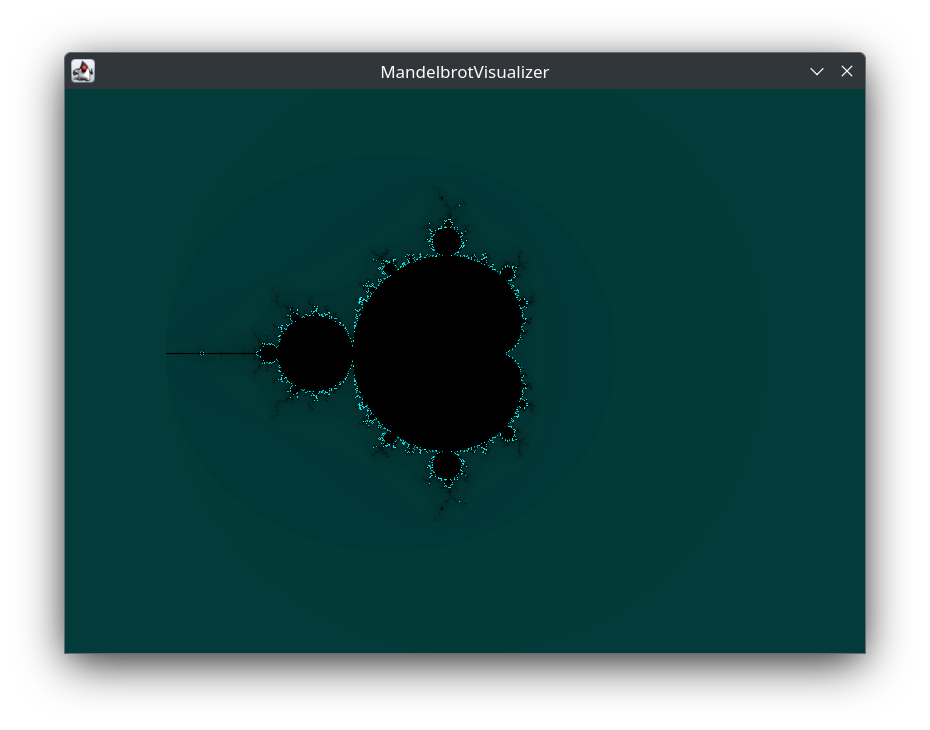
\includegraphics[width=10cm]{Screenshot_20231125_192542.png}\]

    Możemy również uruchomić aplikację z nieco innymi parametrami niż
domyślne:

\begin{Shaded}
\begin{Highlighting}[]
\ExtensionTok{./gradlew}\NormalTok{ run }\AttributeTok{{-}{-}args}\OperatorTok{=}\StringTok{"800 600 {-}700 600 16 8 570 3000 true FIXED\_THREAD\_POOL"}
\end{Highlighting}
\end{Shaded}

tym razem wyświetli się nieco inny obrazek:

\[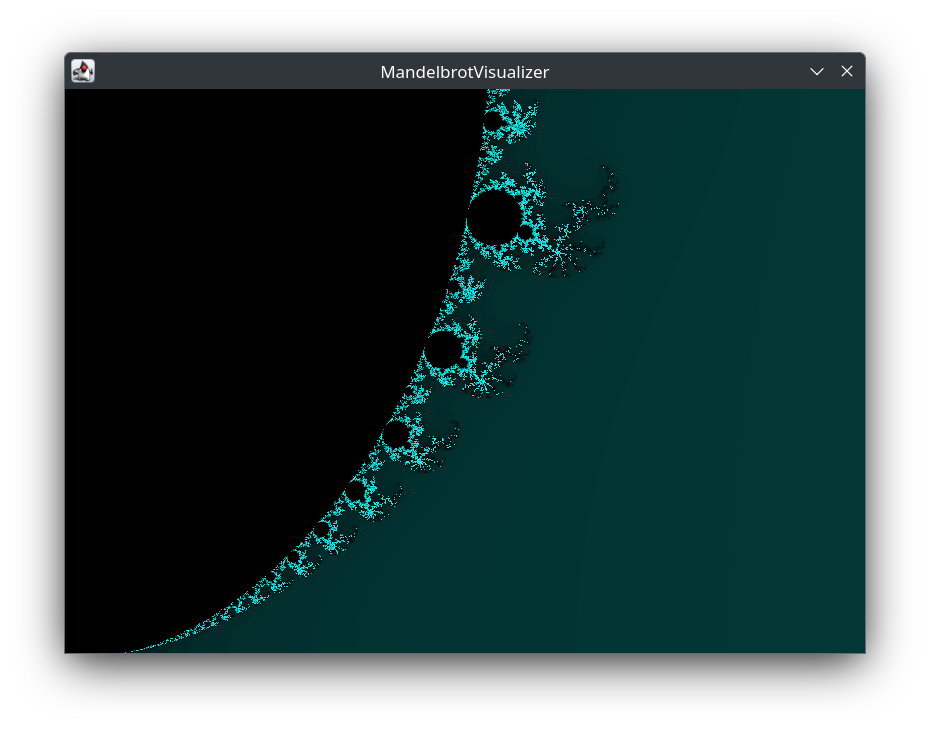
\includegraphics[width=10cm]{Screenshot_20231125_193742.png}\]

    Jak już wspomniano wcześniej, zrównoleglenie obliczeń jest osiągane za
pomocą podziału zbioru pikseli na pewne obszary (chunki), każdy z
których jest obliczany osobno. W powyższej implementacji obraz jest
dzielony na obszary o tej samej wysokości równej wysokości obrazu, tzn.:

\[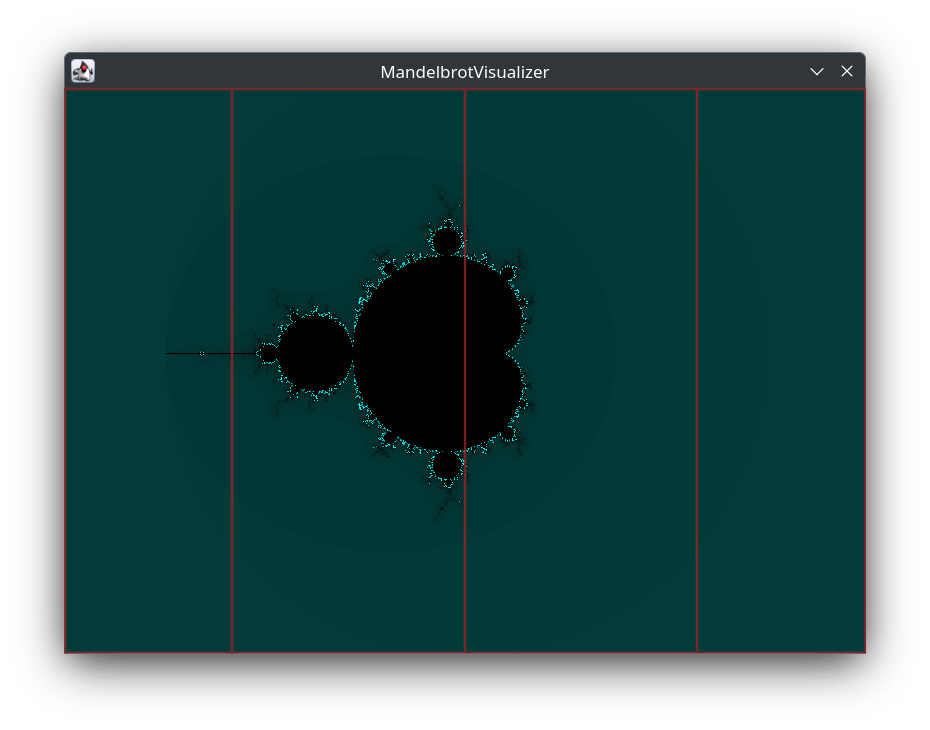
\includegraphics[width=10cm]{Screenshot_20231125_192542_4_chunks.png}\]

jak widać, powyższy obraz został podzielony na 4 \emph{równe} obszary,
każdy z których jest reprezentowany przez osobną instancję
\texttt{MandelbrotChunk} i jest obliczany osobno.

    \hypertarget{wyniki}{%
\section{Wyniki}\label{wyniki}}

W tym rozdziale zostały umieszczone wyniki (pomiary wydajności) w
zależności od implementacji executora i jego parametrów. Wizualne wyniki
zostały zaprezentowane w poprzednim rozdziale.

Podczas testowania został użyty następujący sprzęt i oprogramowanie:

\begin{itemize}
\tightlist
\item
  16 × AMD Ryzen 7 4800H with Radeon Graphics
\item
  Fedora 38, Linux 6.5.9-200.fc38.x86\_64
\item
  openjdk 17.0.8 2023-07-18
\end{itemize}

Dodatkowo, w celach otrzymania i przetwarzania wyników został użyty
język \texttt{python\ 3.11.6} i następujące biblioteki:

\begin{itemize}
\tightlist
\item
  \texttt{matplotlib\ 3.8.1}, służąca do rysowania wykresów
\item
  \texttt{numpy\ 1.26.1}, służąca do obliczeń numerycznych
\item
  \texttt{pandas\ 2.1.3}, służąca do pracy z danymi tabelarycznymi
\end{itemize}

Ponadto, żeby ułatwić proces uruchomienia projektu, skorzystano z
narzędzia \texttt{gradle} (Kotlin DSL).

    \hypertarget{pobieranie-wynikuxf3w}{%
\subsection{Pobieranie wyników}\label{pobieranie-wynikuxf3w}}

W tej części zostaną pobrane wyniki dla wszystkich w/w executorów.

Wszystkie rozwiązania zostaną przetestowane na wspólnych globalnych
(podstawowych) parametrach.

    Tworzę funkcję, która będzie wywoływać program Javowy z określonymi
parametrami i jako wynik zwracać czas wykonania obliczeń wypisany przez
Javowy program:

    \begin{tcolorbox}[breakable, size=fbox, boxrule=1pt, pad at break*=1mm,colback=cellbackground, colframe=cellborder]
\prompt{In}{incolor}{1}{\boxspacing}
\begin{Verbatim}[commandchars=\\\{\}]
\PY{k+kn}{import} \PY{n+nn}{subprocess}
\PY{k+kn}{import} \PY{n+nn}{re}

\PY{k}{def} \PY{n+nf}{run}\PY{p}{(}\PY{n}{width}\PY{p}{:} \PY{n+nb}{int}\PY{p}{,}
        \PY{n}{height}\PY{p}{:} \PY{n+nb}{int}\PY{p}{,}
        \PY{n}{translate\PYZus{}x}\PY{p}{:} \PY{n+nb}{int}\PY{p}{,}
        \PY{n}{translate\PYZus{}y}\PY{p}{:} \PY{n+nb}{int}\PY{p}{,}
        \PY{n}{chunk\PYZus{}count}\PY{p}{:} \PY{n+nb}{int}\PY{p}{,}
        \PY{n}{pool\PYZus{}size}\PY{p}{:} \PY{n+nb}{int}\PY{p}{,}
        \PY{n}{max\PYZus{}iter\PYZus{}count}\PY{p}{:} \PY{n+nb}{int}\PY{p}{,}
        \PY{n}{zoom}\PY{p}{:} \PY{n+nb}{float}\PY{p}{,}
        \PY{n}{executor\PYZus{}type}\PY{p}{:} \PY{n+nb}{str}\PY{p}{,}
        \PY{n}{visualize}\PY{p}{:} \PY{n+nb}{bool} \PY{o}{=} \PY{k+kc}{False}\PY{p}{)} \PY{o}{\PYZhy{}}\PY{o}{\PYZgt{}} \PY{n+nb}{int}\PY{p}{:}
    
    \PY{n}{cmd} \PY{o}{=} \PY{l+s+sa}{f}\PY{l+s+s2}{\PYZdq{}}\PY{l+s+s2}{../tw\PYZhy{}lab8/gradlew run \PYZhy{}\PYZhy{}args=}\PY{l+s+se}{\PYZbs{}\PYZdq{}}\PY{l+s+si}{\PYZob{}}\PY{l+s+s1}{\PYZsq{}}\PY{l+s+si}{\PYZob{}\PYZcb{}}\PY{l+s+s1}{ }\PY{l+s+s1}{\PYZsq{}}\PY{+w}{ }\PY{o}{*}\PY{+w}{ }\PY{l+m+mi}{10}\PY{l+s+si}{\PYZcb{}}\PY{l+s+se}{\PYZbs{}\PYZdq{}}\PY{l+s+s2}{\PYZdq{}}\PY{o}{.}\PY{n}{format}\PY{p}{(}
        \PY{n}{width}\PY{p}{,}
        \PY{n}{height}\PY{p}{,}
        \PY{n}{translate\PYZus{}x}\PY{p}{,}
        \PY{n}{translate\PYZus{}y}\PY{p}{,}
        \PY{n}{chunk\PYZus{}count}\PY{p}{,}
        \PY{n}{pool\PYZus{}size}\PY{p}{,}
        \PY{n}{max\PYZus{}iter\PYZus{}count}\PY{p}{,}
        \PY{n}{zoom}\PY{p}{,}
        \PY{n+nb}{str}\PY{p}{(}\PY{n}{visualize}\PY{p}{)}\PY{o}{.}\PY{n}{lower}\PY{p}{(}\PY{p}{)}\PY{p}{,}
        \PY{n}{executor\PYZus{}type}
    \PY{p}{)}

    \PY{n}{result} \PY{o}{=} \PY{n}{subprocess}\PY{o}{.}\PY{n}{run}\PY{p}{(}
        \PY{p}{[}\PY{l+s+s2}{\PYZdq{}}\PY{l+s+s2}{bash}\PY{l+s+s2}{\PYZdq{}}\PY{p}{,} \PY{l+s+s2}{\PYZdq{}}\PY{l+s+s2}{\PYZhy{}c}\PY{l+s+s2}{\PYZdq{}}\PY{p}{,} \PY{n}{cmd}\PY{p}{]}\PY{p}{,}
        \PY{n}{cwd}\PY{o}{=}\PY{l+s+s2}{\PYZdq{}}\PY{l+s+s2}{../tw\PYZhy{}lab8}\PY{l+s+s2}{\PYZdq{}}\PY{p}{,}
        \PY{n}{stdout}\PY{o}{=}\PY{n}{subprocess}\PY{o}{.}\PY{n}{PIPE}\PY{p}{)}
    
    \PY{k}{return} \PY{n+nb}{int}\PY{p}{(}\PY{n}{re}\PY{o}{.}\PY{n}{search}\PY{p}{(}\PY{l+s+s2}{\PYZdq{}}\PY{l+s+s2}{time=([0\PYZhy{}9]+)}\PY{l+s+s2}{\PYZdq{}}\PY{p}{,} \PY{n+nb}{str}\PY{p}{(}\PY{n}{result}\PY{o}{.}\PY{n}{stdout}\PY{p}{)}\PY{p}{)}\PY{o}{.}\PY{n}{group}\PY{p}{(}\PY{l+m+mi}{1}\PY{p}{)}\PY{p}{)}
\end{Verbatim}
\end{tcolorbox}

    \begin{tcolorbox}[breakable, size=fbox, boxrule=1pt, pad at break*=1mm,colback=cellbackground, colframe=cellborder]
\prompt{In}{incolor}{2}{\boxspacing}
\begin{Verbatim}[commandchars=\\\{\}]
\PY{k+kn}{import} \PY{n+nn}{numpy} \PY{k}{as} \PY{n+nn}{np}

\PY{n}{TO\PYZus{}CENTER} \PY{o}{=} \PY{n}{np}\PY{o}{.}\PY{n}{array}\PY{p}{(}\PY{l+m+mh}{0x80000000}\PY{p}{)}\PY{o}{.}\PY{n}{astype}\PY{p}{(}\PY{n}{np}\PY{o}{.}\PY{n}{int32}\PY{p}{)}
\end{Verbatim}
\end{tcolorbox}

    Tworzę funkcję, która dla podanych argumentów zwraca średni czas
wykonania:

    \begin{tcolorbox}[breakable, size=fbox, boxrule=1pt, pad at break*=1mm,colback=cellbackground, colframe=cellborder]
\prompt{In}{incolor}{3}{\boxspacing}
\begin{Verbatim}[commandchars=\\\{\}]
\PY{k+kn}{import} \PY{n+nn}{numpy} \PY{k}{as} \PY{n+nn}{np}

\PY{k}{def} \PY{n+nf}{run\PYZus{}mean}\PY{p}{(}\PY{n}{n}\PY{p}{:} \PY{n+nb}{int}\PY{p}{,} \PY{o}{*}\PY{o}{*}\PY{n}{kwargs}\PY{p}{)} \PY{o}{\PYZhy{}}\PY{o}{\PYZgt{}} \PY{n+nb}{float}\PY{p}{:}
    \PY{k}{return} \PY{n}{np}\PY{o}{.}\PY{n}{mean}\PY{p}{(}\PY{p}{[}\PY{n}{run}\PY{p}{(}\PY{o}{*}\PY{o}{*}\PY{n}{kwargs}\PY{p}{)} \PY{k}{for} \PY{n}{\PYZus{}} \PY{o+ow}{in} \PY{n+nb}{range}\PY{p}{(}\PY{n}{n}\PY{p}{)}\PY{p}{]}\PY{p}{,} \PY{n}{dtype}\PY{o}{=}\PY{n+nb}{float}\PY{p}{)}
\end{Verbatim}
\end{tcolorbox}

    Definiuję globalne (podstawowe, wspólne) parametry:

    \begin{tcolorbox}[breakable, size=fbox, boxrule=1pt, pad at break*=1mm,colback=cellbackground, colframe=cellborder]
\prompt{In}{incolor}{4}{\boxspacing}
\begin{Verbatim}[commandchars=\\\{\}]
\PY{n}{global\PYZus{}params} \PY{o}{=} \PY{p}{\PYZob{}}
    \PY{l+s+s2}{\PYZdq{}}\PY{l+s+s2}{n}\PY{l+s+s2}{\PYZdq{}}\PY{p}{:} \PY{l+m+mi}{5}\PY{p}{,}
    \PY{l+s+s2}{\PYZdq{}}\PY{l+s+s2}{width}\PY{l+s+s2}{\PYZdq{}}\PY{p}{:} \PY{l+m+mi}{1920}\PY{p}{,}
    \PY{l+s+s2}{\PYZdq{}}\PY{l+s+s2}{height}\PY{l+s+s2}{\PYZdq{}}\PY{p}{:} \PY{l+m+mi}{1080}\PY{p}{,}
    \PY{l+s+s2}{\PYZdq{}}\PY{l+s+s2}{translate\PYZus{}x}\PY{l+s+s2}{\PYZdq{}}\PY{p}{:} \PY{n}{TO\PYZus{}CENTER}\PY{p}{,}
    \PY{l+s+s2}{\PYZdq{}}\PY{l+s+s2}{translate\PYZus{}y}\PY{l+s+s2}{\PYZdq{}}\PY{p}{:} \PY{n}{TO\PYZus{}CENTER}\PY{p}{,}
    \PY{l+s+s2}{\PYZdq{}}\PY{l+s+s2}{chunk\PYZus{}count}\PY{l+s+s2}{\PYZdq{}}\PY{p}{:} \PY{l+m+mi}{16}\PY{p}{,}
    \PY{l+s+s2}{\PYZdq{}}\PY{l+s+s2}{pool\PYZus{}size}\PY{l+s+s2}{\PYZdq{}}\PY{p}{:} \PY{l+m+mi}{8}\PY{p}{,}
    \PY{l+s+s2}{\PYZdq{}}\PY{l+s+s2}{max\PYZus{}iter\PYZus{}count}\PY{l+s+s2}{\PYZdq{}}\PY{p}{:} \PY{l+m+mi}{4096}\PY{p}{,}
    \PY{l+s+s2}{\PYZdq{}}\PY{l+s+s2}{zoom}\PY{l+s+s2}{\PYZdq{}}\PY{p}{:} \PY{l+m+mi}{300}\PY{p}{,}
    \PY{l+s+s2}{\PYZdq{}}\PY{l+s+s2}{visualize}\PY{l+s+s2}{\PYZdq{}}\PY{p}{:} \PY{k+kc}{False}\PY{p}{,}
    \PY{l+s+s2}{\PYZdq{}}\PY{l+s+s2}{executor\PYZus{}type}\PY{l+s+s2}{\PYZdq{}}\PY{p}{:} \PY{l+s+s2}{\PYZdq{}}\PY{l+s+s2}{FIXED\PYZus{}THREAD\PYZus{}POOL}\PY{l+s+s2}{\PYZdq{}}
\PY{p}{\PYZcb{}}
\end{Verbatim}
\end{tcolorbox}

    Tworzę funkcję tworzącą nowy zbiór (słownik) parametrów w oparciu o
\texttt{global\_params}:

    \begin{tcolorbox}[breakable, size=fbox, boxrule=1pt, pad at break*=1mm,colback=cellbackground, colframe=cellborder]
\prompt{In}{incolor}{5}{\boxspacing}
\begin{Verbatim}[commandchars=\\\{\}]
\PY{k+kn}{from} \PY{n+nn}{typing} \PY{k+kn}{import} \PY{n}{Any}

\PY{k}{def} \PY{n+nf}{get\PYZus{}params}\PY{p}{(}\PY{o}{*}\PY{o}{*}\PY{n}{kwargs}\PY{p}{)} \PY{o}{\PYZhy{}}\PY{o}{\PYZgt{}} \PY{n+nb}{dict}\PY{p}{[}\PY{n+nb}{str}\PY{p}{,} \PY{n}{Any}\PY{p}{]}\PY{p}{:}
    \PY{k}{return} \PY{n}{global\PYZus{}params} \PY{o}{|} \PY{n}{kwargs}
\end{Verbatim}
\end{tcolorbox}

    Teraz stworzę zbiór parametrów testowych. Warto zauważyć, że różne
executory są czułe na zmiany różnych parametrów. Na przykład, w
przypadku \texttt{SINGLE\_THREAD} nie ma żadnego sensu zmieniać ani
rozmiar puli wątków ani liczby chunków - wszystko jest i tak obliczane w
jednym wątku, więc zmiana rozmiaru puli w cale nie będzie miała żadnego
wpływu na wyniki, a zmiana liczby chunków (w granicach rozsądku) prawie
nie będzie miała wpływu na ostateczny wynik.

Dla poszczególnych executorów zostaną przetestowane zmiany nastepujących
parametrów:

\begin{itemize}
\tightlist
\item
  \texttt{SINGLE\_THREAD}:

  \begin{itemize}
  \tightlist
  \item
    \texttt{chunk\_count}
  \end{itemize}
\item
  \texttt{FIXED\_THREAD\_POOL}:

  \begin{itemize}
  \tightlist
  \item
    \texttt{chunk\_count}
  \item
    \texttt{pool\_size}
  \end{itemize}
\item
  \texttt{CACHED\_THREAD\_POOL}:

  \begin{itemize}
  \tightlist
  \item
    \texttt{chunk\_count}
  \end{itemize}
\item
  \texttt{WORK\_STEALING\_POOL}:

  \begin{itemize}
  \tightlist
  \item
    \texttt{chunk\_count}
  \end{itemize}
\end{itemize}

    \begin{tcolorbox}[breakable, size=fbox, boxrule=1pt, pad at break*=1mm,colback=cellbackground, colframe=cellborder]
\prompt{In}{incolor}{6}{\boxspacing}
\begin{Verbatim}[commandchars=\\\{\}]
\PY{n}{chunk\PYZus{}count\PYZus{}values} \PY{o}{=} \PY{n}{np}\PY{o}{.}\PY{n}{concatenate}\PY{p}{(}\PY{p}{[}\PY{p}{[}\PY{l+m+mi}{1}\PY{p}{]}\PY{p}{,} \PY{n}{np}\PY{o}{.}\PY{n}{arange}\PY{p}{(}\PY{l+m+mi}{2}\PY{p}{,} \PY{l+m+mi}{31}\PY{p}{,} \PY{l+m+mi}{4}\PY{p}{)}\PY{p}{]}\PY{p}{)}
\PY{n}{pool\PYZus{}size\PYZus{}values} \PY{o}{=} \PY{n}{np}\PY{o}{.}\PY{n}{concatenate}\PY{p}{(}\PY{p}{[}\PY{p}{[}\PY{l+m+mi}{1}\PY{p}{]}\PY{p}{,} \PY{n}{np}\PY{o}{.}\PY{n}{arange}\PY{p}{(}\PY{l+m+mi}{2}\PY{p}{,} \PY{l+m+mi}{31}\PY{p}{,} \PY{l+m+mi}{4}\PY{p}{)}\PY{p}{]}\PY{p}{)}
\end{Verbatim}
\end{tcolorbox}

    Tworzę funkcje generujące parametry:

    \begin{tcolorbox}[breakable, size=fbox, boxrule=1pt, pad at break*=1mm,colback=cellbackground, colframe=cellborder]
\prompt{In}{incolor}{7}{\boxspacing}
\begin{Verbatim}[commandchars=\\\{\}]
\PY{k+kn}{from} \PY{n+nn}{typing} \PY{k+kn}{import} \PY{n}{Iterable}

\PY{k}{def} \PY{n+nf}{param\PYZus{}generator\PYZus{}1d}\PY{p}{(}\PY{n}{key}\PY{p}{:} \PY{n+nb}{str}\PY{p}{,} \PY{n}{values}\PY{p}{:} \PY{n}{Iterable}\PY{p}{[}\PY{n}{Any}\PY{p}{]}\PY{p}{,} \PY{o}{*}\PY{o}{*}\PY{n}{const\PYZus{}params}\PY{p}{)} \PY{o}{\PYZhy{}}\PY{o}{\PYZgt{}} \PY{n}{Iterable}\PY{p}{[}\PY{n+nb}{dict}\PY{p}{[}\PY{n+nb}{str}\PY{p}{,} \PY{n}{Any}\PY{p}{]}\PY{p}{]}\PY{p}{:}
    \PY{k}{for} \PY{n}{val} \PY{o+ow}{in} \PY{n}{values}\PY{p}{:}
        \PY{k}{yield} \PY{n}{get\PYZus{}params}\PY{p}{(}\PY{o}{*}\PY{o}{*}\PY{p}{(}\PY{p}{\PYZob{}}\PY{n}{key}\PY{p}{:} \PY{n}{val}\PY{p}{\PYZcb{}} \PY{o}{|} \PY{n}{const\PYZus{}params}\PY{p}{)}\PY{p}{)}
\end{Verbatim}
\end{tcolorbox}

    \begin{tcolorbox}[breakable, size=fbox, boxrule=1pt, pad at break*=1mm,colback=cellbackground, colframe=cellborder]
\prompt{In}{incolor}{8}{\boxspacing}
\begin{Verbatim}[commandchars=\\\{\}]
\PY{k+kn}{from} \PY{n+nn}{typing} \PY{k+kn}{import} \PY{n}{Iterable}

\PY{k}{def} \PY{n+nf}{param\PYZus{}generator\PYZus{}2d}\PY{p}{(}
        \PY{n}{key0}\PY{p}{:} \PY{n+nb}{str}\PY{p}{,} \PY{n}{values0}\PY{p}{:} \PY{n}{Iterable}\PY{p}{[}\PY{n}{Any}\PY{p}{]}\PY{p}{,}
        \PY{n}{key1}\PY{p}{:} \PY{n+nb}{str}\PY{p}{,} \PY{n}{values1}\PY{p}{:} \PY{n}{Iterable}\PY{p}{[}\PY{n}{Any}\PY{p}{]}\PY{p}{,}
        \PY{o}{*}\PY{o}{*}\PY{n}{const\PYZus{}params}\PY{p}{)} \PY{o}{\PYZhy{}}\PY{o}{\PYZgt{}} \PY{n}{Iterable}\PY{p}{[}\PY{n+nb}{dict}\PY{p}{[}\PY{n+nb}{str}\PY{p}{,} \PY{n}{Any}\PY{p}{]}\PY{p}{]}\PY{p}{:}
    \PY{k}{for} \PY{n}{val0} \PY{o+ow}{in} \PY{n}{values0}\PY{p}{:}
        \PY{k}{for} \PY{n}{val1} \PY{o+ow}{in} \PY{n}{values1}\PY{p}{:}
            \PY{k}{yield} \PY{n}{get\PYZus{}params}\PY{p}{(}\PY{o}{*}\PY{o}{*}\PY{p}{(}\PY{p}{\PYZob{}}\PY{n}{key0}\PY{p}{:} \PY{n}{val0}\PY{p}{,} \PY{n}{key1}\PY{p}{:} \PY{n}{val1}\PY{p}{\PYZcb{}} \PY{o}{|} \PY{n}{const\PYZus{}params}\PY{p}{)}\PY{p}{)}
\end{Verbatim}
\end{tcolorbox}

    Tworzę funkcję wykonującą pomiary dla podanego zbioru parametrów i
zwracającą wyniki:

    \begin{tcolorbox}[breakable, size=fbox, boxrule=1pt, pad at break*=1mm,colback=cellbackground, colframe=cellborder]
\prompt{In}{incolor}{9}{\boxspacing}
\begin{Verbatim}[commandchars=\\\{\}]
\PY{k+kn}{import} \PY{n+nn}{pandas} \PY{k}{as} \PY{n+nn}{pd}

\PY{k}{def} \PY{n+nf}{runner}\PY{p}{(}\PY{n}{param\PYZus{}set}\PY{p}{:} \PY{n}{Iterable}\PY{p}{[}\PY{n+nb}{dict}\PY{p}{[}\PY{n+nb}{str}\PY{p}{,} \PY{n}{Any}\PY{p}{]}\PY{p}{]}\PY{p}{,} \PY{n}{columns}\PY{p}{:} \PY{n+nb}{list}\PY{p}{[}\PY{n+nb}{str}\PY{p}{]}\PY{p}{)} \PY{o}{\PYZhy{}}\PY{o}{\PYZgt{}} \PY{n}{pd}\PY{o}{.}\PY{n}{DataFrame}\PY{p}{:}
    \PY{n}{result} \PY{o}{=} \PY{n}{pd}\PY{o}{.}\PY{n}{DataFrame}\PY{p}{(}\PY{p}{)}

    \PY{k}{for} \PY{n}{params} \PY{o+ow}{in} \PY{n}{param\PYZus{}set}\PY{p}{:}
        \PY{n}{time} \PY{o}{=} \PY{n}{run\PYZus{}mean}\PY{p}{(}\PY{o}{*}\PY{o}{*}\PY{n}{params}\PY{p}{)}
        \PY{n}{row} \PY{o}{=} \PY{n}{pd}\PY{o}{.}\PY{n}{DataFrame}\PY{p}{(}\PY{n+nb}{dict}\PY{p}{(}\PY{p}{[}\PY{p}{(}\PY{n}{col}\PY{p}{,} \PY{n}{params}\PY{p}{[}\PY{n}{col}\PY{p}{]}\PY{p}{)} \PY{k}{for} \PY{n}{col} \PY{o+ow}{in} \PY{n}{columns}\PY{p}{]} \PY{o}{+} \PY{p}{[}\PY{p}{(}\PY{l+s+s2}{\PYZdq{}}\PY{l+s+s2}{time}\PY{l+s+s2}{\PYZdq{}}\PY{p}{,} \PY{n}{time}\PY{p}{)}\PY{p}{]}\PY{p}{)}\PY{p}{,} \PY{n}{index}\PY{o}{=}\PY{p}{[}\PY{n+nb}{len}\PY{p}{(}\PY{n}{result}\PY{p}{)}\PY{p}{]}\PY{p}{)}
        \PY{n}{result} \PY{o}{=} \PY{n}{pd}\PY{o}{.}\PY{n}{concat}\PY{p}{(}\PY{p}{[}\PY{n}{result}\PY{p}{,} \PY{n}{row}\PY{p}{]}\PY{p}{)}

    \PY{k}{return} \PY{n}{result}
\end{Verbatim}
\end{tcolorbox}

    Wykonuję pomiary:

    \begin{tcolorbox}[breakable, size=fbox, boxrule=1pt, pad at break*=1mm,colback=cellbackground, colframe=cellborder]
\prompt{In}{incolor}{10}{\boxspacing}
\begin{Verbatim}[commandchars=\\\{\}]
\PY{n+nb}{print}\PY{p}{(}\PY{l+s+s2}{\PYZdq{}}\PY{l+s+s2}{single\PYZus{}thread\PYZus{}df}\PY{l+s+s2}{\PYZdq{}}\PY{p}{)}
\PY{n}{single\PYZus{}thread\PYZus{}df} \PY{o}{=} \PY{n}{runner}\PY{p}{(}\PY{n}{param\PYZus{}generator\PYZus{}1d}\PY{p}{(}
    \PY{l+s+s2}{\PYZdq{}}\PY{l+s+s2}{chunk\PYZus{}count}\PY{l+s+s2}{\PYZdq{}}\PY{p}{,} \PY{n}{chunk\PYZus{}count\PYZus{}values}\PY{p}{,}
    \PY{n}{executor\PYZus{}type}\PY{o}{=}\PY{l+s+s2}{\PYZdq{}}\PY{l+s+s2}{SINGLE\PYZus{}THREAD}\PY{l+s+s2}{\PYZdq{}}\PY{p}{)}\PY{p}{,} \PY{p}{[}\PY{l+s+s2}{\PYZdq{}}\PY{l+s+s2}{chunk\PYZus{}count}\PY{l+s+s2}{\PYZdq{}}\PY{p}{]}\PY{p}{)}

\PY{n+nb}{print}\PY{p}{(}\PY{l+s+s2}{\PYZdq{}}\PY{l+s+s2}{fixed\PYZus{}thread\PYZus{}pool\PYZus{}df}\PY{l+s+s2}{\PYZdq{}}\PY{p}{)}
\PY{n}{fixed\PYZus{}thread\PYZus{}pool\PYZus{}df} \PY{o}{=} \PY{n}{runner}\PY{p}{(}\PY{n}{param\PYZus{}generator\PYZus{}2d}\PY{p}{(}
    \PY{n}{key0}\PY{o}{=}\PY{l+s+s2}{\PYZdq{}}\PY{l+s+s2}{chunk\PYZus{}count}\PY{l+s+s2}{\PYZdq{}}\PY{p}{,} \PY{n}{values0}\PY{o}{=}\PY{n}{chunk\PYZus{}count\PYZus{}values}\PY{p}{,}
    \PY{n}{key1}\PY{o}{=}\PY{l+s+s2}{\PYZdq{}}\PY{l+s+s2}{pool\PYZus{}size}\PY{l+s+s2}{\PYZdq{}}\PY{p}{,} \PY{n}{values1}\PY{o}{=}\PY{n}{pool\PYZus{}size\PYZus{}values}\PY{p}{,}
    \PY{n}{executor\PYZus{}type}\PY{o}{=}\PY{l+s+s2}{\PYZdq{}}\PY{l+s+s2}{FIXED\PYZus{}THREAD\PYZus{}POOL}\PY{l+s+s2}{\PYZdq{}}\PY{p}{)}\PY{p}{,} \PY{p}{[}\PY{l+s+s2}{\PYZdq{}}\PY{l+s+s2}{chunk\PYZus{}count}\PY{l+s+s2}{\PYZdq{}}\PY{p}{,} \PY{l+s+s2}{\PYZdq{}}\PY{l+s+s2}{pool\PYZus{}size}\PY{l+s+s2}{\PYZdq{}}\PY{p}{]}\PY{p}{)}

\PY{n+nb}{print}\PY{p}{(}\PY{l+s+s2}{\PYZdq{}}\PY{l+s+s2}{cached\PYZus{}thread\PYZus{}pool\PYZus{}df}\PY{l+s+s2}{\PYZdq{}}\PY{p}{)}
\PY{n}{cached\PYZus{}thread\PYZus{}pool\PYZus{}df} \PY{o}{=} \PY{n}{runner}\PY{p}{(}\PY{n}{param\PYZus{}generator\PYZus{}1d}\PY{p}{(}
    \PY{l+s+s2}{\PYZdq{}}\PY{l+s+s2}{chunk\PYZus{}count}\PY{l+s+s2}{\PYZdq{}}\PY{p}{,} \PY{n}{chunk\PYZus{}count\PYZus{}values}\PY{p}{,}
    \PY{n}{executor\PYZus{}type}\PY{o}{=}\PY{l+s+s2}{\PYZdq{}}\PY{l+s+s2}{CACHED\PYZus{}THREAD\PYZus{}POOL}\PY{l+s+s2}{\PYZdq{}}\PY{p}{)}\PY{p}{,} \PY{p}{[}\PY{l+s+s2}{\PYZdq{}}\PY{l+s+s2}{chunk\PYZus{}count}\PY{l+s+s2}{\PYZdq{}}\PY{p}{]}\PY{p}{)}

\PY{n+nb}{print}\PY{p}{(}\PY{l+s+s2}{\PYZdq{}}\PY{l+s+s2}{work\PYZus{}stealing\PYZus{}pool\PYZus{}df}\PY{l+s+s2}{\PYZdq{}}\PY{p}{)}
\PY{n}{work\PYZus{}stealing\PYZus{}pool\PYZus{}df} \PY{o}{=} \PY{n}{runner}\PY{p}{(}\PY{n}{param\PYZus{}generator\PYZus{}1d}\PY{p}{(}
    \PY{l+s+s2}{\PYZdq{}}\PY{l+s+s2}{chunk\PYZus{}count}\PY{l+s+s2}{\PYZdq{}}\PY{p}{,} \PY{n}{chunk\PYZus{}count\PYZus{}values}\PY{p}{,}
    \PY{n}{executor\PYZus{}type}\PY{o}{=}\PY{l+s+s2}{\PYZdq{}}\PY{l+s+s2}{WORK\PYZus{}STEALING\PYZus{}POOL}\PY{l+s+s2}{\PYZdq{}}\PY{p}{)}\PY{p}{,} \PY{p}{[}\PY{l+s+s2}{\PYZdq{}}\PY{l+s+s2}{chunk\PYZus{}count}\PY{l+s+s2}{\PYZdq{}}\PY{p}{]}\PY{p}{)}
\end{Verbatim}
\end{tcolorbox}

    \begin{Verbatim}[commandchars=\\\{\}]
single\_thread\_df
fixed\_thread\_pool\_df
cached\_thread\_pool\_df
work\_stealing\_pool\_df
    \end{Verbatim}

    \begin{tcolorbox}[breakable, size=fbox, boxrule=1pt, pad at break*=1mm,colback=cellbackground, colframe=cellborder]
\prompt{In}{incolor}{11}{\boxspacing}
\begin{Verbatim}[commandchars=\\\{\}]
\PY{n}{single\PYZus{}thread\PYZus{}df}\PY{o}{.}\PY{n}{head}\PY{p}{(}\PY{p}{)}
\end{Verbatim}
\end{tcolorbox}

            \begin{tcolorbox}[breakable, size=fbox, boxrule=.5pt, pad at break*=1mm, opacityfill=0]
\prompt{Out}{outcolor}{11}{\boxspacing}
\begin{Verbatim}[commandchars=\\\{\}]
   chunk\_count    time
0            1  1846.8
1            2  2394.8
2            6  1811.0
3           10  1415.2
4           14  1862.0
\end{Verbatim}
\end{tcolorbox}
        
    \begin{tcolorbox}[breakable, size=fbox, boxrule=1pt, pad at break*=1mm,colback=cellbackground, colframe=cellborder]
\prompt{In}{incolor}{12}{\boxspacing}
\begin{Verbatim}[commandchars=\\\{\}]
\PY{n}{fixed\PYZus{}thread\PYZus{}pool\PYZus{}df}\PY{o}{.}\PY{n}{head}\PY{p}{(}\PY{p}{)}
\end{Verbatim}
\end{tcolorbox}

            \begin{tcolorbox}[breakable, size=fbox, boxrule=.5pt, pad at break*=1mm, opacityfill=0]
\prompt{Out}{outcolor}{12}{\boxspacing}
\begin{Verbatim}[commandchars=\\\{\}]
   chunk\_count  pool\_size    time
0            1          1  2272.4
1            1          2  2274.8
2            1          6  2487.0
3            1         10  2496.6
4            1         14  2486.6
\end{Verbatim}
\end{tcolorbox}
        
    \begin{tcolorbox}[breakable, size=fbox, boxrule=1pt, pad at break*=1mm,colback=cellbackground, colframe=cellborder]
\prompt{In}{incolor}{13}{\boxspacing}
\begin{Verbatim}[commandchars=\\\{\}]
\PY{n}{cached\PYZus{}thread\PYZus{}pool\PYZus{}df}\PY{o}{.}\PY{n}{head}\PY{p}{(}\PY{p}{)}
\end{Verbatim}
\end{tcolorbox}

            \begin{tcolorbox}[breakable, size=fbox, boxrule=.5pt, pad at break*=1mm, opacityfill=0]
\prompt{Out}{outcolor}{13}{\boxspacing}
\begin{Verbatim}[commandchars=\\\{\}]
   chunk\_count    time
0            1  2270.4
1            2  1661.4
2            6  1695.4
3           10  1398.8
4           14  1109.4
\end{Verbatim}
\end{tcolorbox}
        
    \begin{tcolorbox}[breakable, size=fbox, boxrule=1pt, pad at break*=1mm,colback=cellbackground, colframe=cellborder]
\prompt{In}{incolor}{14}{\boxspacing}
\begin{Verbatim}[commandchars=\\\{\}]
\PY{n}{work\PYZus{}stealing\PYZus{}pool\PYZus{}df}\PY{o}{.}\PY{n}{head}\PY{p}{(}\PY{p}{)}
\end{Verbatim}
\end{tcolorbox}

            \begin{tcolorbox}[breakable, size=fbox, boxrule=.5pt, pad at break*=1mm, opacityfill=0]
\prompt{Out}{outcolor}{14}{\boxspacing}
\begin{Verbatim}[commandchars=\\\{\}]
   chunk\_count    time
0            1  2487.2
1            2  1830.2
2            6  1702.8
3           10  1408.0
4           14  1126.8
\end{Verbatim}
\end{tcolorbox}
        
    \begin{tcolorbox}[breakable, size=fbox, boxrule=1pt, pad at break*=1mm,colback=cellbackground, colframe=cellborder]
\prompt{In}{incolor}{15}{\boxspacing}
\begin{Verbatim}[commandchars=\\\{\}]
\PY{n}{mean\PYZus{}times} \PY{o}{=} \PY{n}{pd}\PY{o}{.}\PY{n}{DataFrame}\PY{p}{(}\PY{p}{\PYZob{}}
    \PY{l+s+s2}{\PYZdq{}}\PY{l+s+s2}{name}\PY{l+s+s2}{\PYZdq{}}\PY{p}{:} \PY{p}{[}
        \PY{l+s+s2}{\PYZdq{}}\PY{l+s+s2}{single\PYZus{}thread\PYZus{}df}\PY{l+s+s2}{\PYZdq{}}\PY{p}{,}
        \PY{l+s+s2}{\PYZdq{}}\PY{l+s+s2}{fixed\PYZus{}thread\PYZus{}pool\PYZus{}df}\PY{l+s+s2}{\PYZdq{}}\PY{p}{,}
        \PY{l+s+s2}{\PYZdq{}}\PY{l+s+s2}{cached\PYZus{}thread\PYZus{}pool\PYZus{}df}\PY{l+s+s2}{\PYZdq{}}\PY{p}{,}
        \PY{l+s+s2}{\PYZdq{}}\PY{l+s+s2}{work\PYZus{}stealing\PYZus{}pool\PYZus{}df}\PY{l+s+s2}{\PYZdq{}}
    \PY{p}{]}\PY{p}{,}
    \PY{l+s+s2}{\PYZdq{}}\PY{l+s+s2}{time}\PY{l+s+s2}{\PYZdq{}}\PY{p}{:} \PY{p}{[}
        \PY{n}{np}\PY{o}{.}\PY{n}{mean}\PY{p}{(}\PY{n}{single\PYZus{}thread\PYZus{}df}\PY{p}{[}\PY{l+s+s2}{\PYZdq{}}\PY{l+s+s2}{time}\PY{l+s+s2}{\PYZdq{}}\PY{p}{]}\PY{p}{)}\PY{p}{,}
        \PY{n}{np}\PY{o}{.}\PY{n}{mean}\PY{p}{(}\PY{n}{fixed\PYZus{}thread\PYZus{}pool\PYZus{}df}\PY{p}{[}\PY{l+s+s2}{\PYZdq{}}\PY{l+s+s2}{time}\PY{l+s+s2}{\PYZdq{}}\PY{p}{]}\PY{p}{)}\PY{p}{,}
        \PY{n}{np}\PY{o}{.}\PY{n}{mean}\PY{p}{(}\PY{n}{cached\PYZus{}thread\PYZus{}pool\PYZus{}df}\PY{p}{[}\PY{l+s+s2}{\PYZdq{}}\PY{l+s+s2}{time}\PY{l+s+s2}{\PYZdq{}}\PY{p}{]}\PY{p}{)}\PY{p}{,}
        \PY{n}{np}\PY{o}{.}\PY{n}{mean}\PY{p}{(}\PY{n}{work\PYZus{}stealing\PYZus{}pool\PYZus{}df}\PY{p}{[}\PY{l+s+s2}{\PYZdq{}}\PY{l+s+s2}{time}\PY{l+s+s2}{\PYZdq{}}\PY{p}{]}\PY{p}{)}
    \PY{p}{]}
\PY{p}{\PYZcb{}}\PY{p}{)}
\end{Verbatim}
\end{tcolorbox}

    \begin{tcolorbox}[breakable, size=fbox, boxrule=1pt, pad at break*=1mm,colback=cellbackground, colframe=cellborder]
\prompt{In}{incolor}{16}{\boxspacing}
\begin{Verbatim}[commandchars=\\\{\}]
\PY{n}{mean\PYZus{}times}
\end{Verbatim}
\end{tcolorbox}

            \begin{tcolorbox}[breakable, size=fbox, boxrule=.5pt, pad at break*=1mm, opacityfill=0]
\prompt{Out}{outcolor}{16}{\boxspacing}
\begin{Verbatim}[commandchars=\\\{\}]
                    name         time
0       single\_thread\_df  1695.955556
1   fixed\_thread\_pool\_df  1287.562963
2  cached\_thread\_pool\_df  1247.933333
3  work\_stealing\_pool\_df  1294.577778
\end{Verbatim}
\end{tcolorbox}
        
    Mamy już dane, a więc możemy przejść do rysowania wykresów.

    \hypertarget{wykresy}{%
\subsection{Wykresy}\label{wykresy}}

    \begin{tcolorbox}[breakable, size=fbox, boxrule=1pt, pad at break*=1mm,colback=cellbackground, colframe=cellborder]
\prompt{In}{incolor}{17}{\boxspacing}
\begin{Verbatim}[commandchars=\\\{\}]
\PY{o}{\PYZpc{}}\PY{k}{config} InlineBackend.figure\PYZus{}formats = [\PYZsq{}svg\PYZsq{}]
\end{Verbatim}
\end{tcolorbox}

    Tworzę funkcje służące do rysowania 2D oraz 3D wykresów:

    \begin{tcolorbox}[breakable, size=fbox, boxrule=1pt, pad at break*=1mm,colback=cellbackground, colframe=cellborder]
\prompt{In}{incolor}{18}{\boxspacing}
\begin{Verbatim}[commandchars=\\\{\}]
\PY{k}{def} \PY{n+nf}{plot2d}\PY{p}{(}\PY{n}{df}\PY{p}{:} \PY{n}{pd}\PY{o}{.}\PY{n}{DataFrame}\PY{p}{,} \PY{n}{title}\PY{p}{:} \PY{n+nb}{str}\PY{p}{,} \PY{n}{x}\PY{p}{:} \PY{n+nb}{str} \PY{o}{=} \PY{l+s+s2}{\PYZdq{}}\PY{l+s+s2}{chunk\PYZus{}count}\PY{l+s+s2}{\PYZdq{}}\PY{p}{)}\PY{p}{:}
    \PY{n}{df}\PY{o}{.}\PY{n}{plot}\PY{p}{(}\PY{n}{kind}\PY{o}{=}\PY{l+s+s2}{\PYZdq{}}\PY{l+s+s2}{bar}\PY{l+s+s2}{\PYZdq{}}\PY{p}{,} \PY{n}{x}\PY{o}{=}\PY{n}{x}\PY{p}{,} \PY{n}{ylabel}\PY{o}{=}\PY{l+s+s2}{\PYZdq{}}\PY{l+s+s2}{time, \PYZdl{}[ms]\PYZdl{}}\PY{l+s+s2}{\PYZdq{}}\PY{p}{,} \PY{n}{title}\PY{o}{=}\PY{n}{title}\PY{p}{)}
\end{Verbatim}
\end{tcolorbox}

    \begin{tcolorbox}[breakable, size=fbox, boxrule=1pt, pad at break*=1mm,colback=cellbackground, colframe=cellborder]
\prompt{In}{incolor}{19}{\boxspacing}
\begin{Verbatim}[commandchars=\\\{\}]
\PY{k+kn}{import} \PY{n+nn}{matplotlib}\PY{n+nn}{.}\PY{n+nn}{pyplot} \PY{k}{as} \PY{n+nn}{plt}

\PY{k}{def} \PY{n+nf}{plot3d}\PY{p}{(}\PY{n}{df}\PY{p}{:} \PY{n}{pd}\PY{o}{.}\PY{n}{DataFrame}\PY{p}{,} \PY{n}{title}\PY{p}{:} \PY{n+nb}{str}\PY{p}{,} \PY{n}{x}\PY{p}{:} \PY{n+nb}{str} \PY{o}{=} \PY{l+s+s2}{\PYZdq{}}\PY{l+s+s2}{chunk\PYZus{}count}\PY{l+s+s2}{\PYZdq{}}\PY{p}{,} \PY{n}{y}\PY{p}{:} \PY{n+nb}{str} \PY{o}{=} \PY{l+s+s2}{\PYZdq{}}\PY{l+s+s2}{pool\PYZus{}size}\PY{l+s+s2}{\PYZdq{}}\PY{p}{,} \PY{n}{z}\PY{p}{:} \PY{n+nb}{str} \PY{o}{=} \PY{l+s+s2}{\PYZdq{}}\PY{l+s+s2}{time}\PY{l+s+s2}{\PYZdq{}}\PY{p}{,} \PY{n}{azim}\PY{p}{:} \PY{n+nb}{float} \PY{o}{=} \PY{o}{\PYZhy{}}\PY{l+m+mi}{45}\PY{p}{)}\PY{p}{:}
    \PY{c+c1}{\PYZsh{} set up the figure and axes}
    \PY{n}{fig} \PY{o}{=} \PY{n}{plt}\PY{o}{.}\PY{n}{figure}\PY{p}{(}\PY{n}{figsize}\PY{o}{=}\PY{p}{(}\PY{l+m+mi}{16}\PY{p}{,} \PY{l+m+mi}{16}\PY{p}{)}\PY{p}{)}
    \PY{n}{ax} \PY{o}{=} \PY{n}{fig}\PY{o}{.}\PY{n}{add\PYZus{}subplot}\PY{p}{(}\PY{l+m+mi}{111}\PY{p}{,} \PY{n}{projection}\PY{o}{=}\PY{l+s+s1}{\PYZsq{}}\PY{l+s+s1}{3d}\PY{l+s+s1}{\PYZsq{}}\PY{p}{)}

    \PY{n}{ax}\PY{o}{.}\PY{n}{view\PYZus{}init}\PY{p}{(}\PY{n}{azim}\PY{o}{=}\PY{n}{azim}\PY{p}{)}

    \PY{n}{width} \PY{o}{=} \PY{l+m+mf}{3.5}
    \PY{n}{depth} \PY{o}{=} \PY{l+m+mf}{3.5}

    \PY{n}{ax}\PY{o}{.}\PY{n}{bar3d}\PY{p}{(}\PY{n}{df}\PY{p}{[}\PY{n}{x}\PY{p}{]}\PY{p}{,} \PY{n}{df}\PY{p}{[}\PY{n}{y}\PY{p}{]}\PY{p}{,} \PY{n}{np}\PY{o}{.}\PY{n}{zeros\PYZus{}like}\PY{p}{(}\PY{n}{df}\PY{p}{[}\PY{n}{z}\PY{p}{]}\PY{p}{)}\PY{p}{,} \PY{n}{width}\PY{p}{,} \PY{n}{depth}\PY{p}{,} \PY{n}{df}\PY{p}{[}\PY{n}{z}\PY{p}{]}\PY{p}{,} \PY{n}{shade}\PY{o}{=}\PY{k+kc}{True}\PY{p}{)}
    \PY{n}{ax}\PY{o}{.}\PY{n}{set\PYZus{}title}\PY{p}{(}\PY{n}{title}\PY{p}{)}
    \PY{n}{ax}\PY{o}{.}\PY{n}{set\PYZus{}xlabel}\PY{p}{(}\PY{n}{x}\PY{p}{)}
    \PY{n}{ax}\PY{o}{.}\PY{n}{set\PYZus{}ylabel}\PY{p}{(}\PY{n}{y}\PY{p}{)}
    \PY{n}{ax}\PY{o}{.}\PY{n}{set\PYZus{}zlabel}\PY{p}{(}\PY{n}{z}\PY{p}{)}

    \PY{n}{plt}\PY{o}{.}\PY{n}{show}\PY{p}{(}\PY{p}{)}
\end{Verbatim}
\end{tcolorbox}

    Wyświetlam wykresy pokazujące zależności od poszczególnych zmiennych:

    \begin{tcolorbox}[breakable, size=fbox, boxrule=1pt, pad at break*=1mm,colback=cellbackground, colframe=cellborder]
\prompt{In}{incolor}{20}{\boxspacing}
\begin{Verbatim}[commandchars=\\\{\}]
\PY{n}{plot2d}\PY{p}{(}\PY{n}{single\PYZus{}thread\PYZus{}df}\PY{p}{,} \PY{l+s+s2}{\PYZdq{}}\PY{l+s+s2}{single\PYZus{}thread\PYZus{}df}\PY{l+s+s2}{\PYZdq{}}\PY{p}{)}
\end{Verbatim}
\end{tcolorbox}

    \begin{center}
    \adjustimage{max size={0.9\linewidth}{0.9\paperheight}}{output_44_0.pdf}
    \end{center}
    { \hspace*{\fill} \\}
    
    \begin{tcolorbox}[breakable, size=fbox, boxrule=1pt, pad at break*=1mm,colback=cellbackground, colframe=cellborder]
\prompt{In}{incolor}{21}{\boxspacing}
\begin{Verbatim}[commandchars=\\\{\}]
\PY{n}{plot2d}\PY{p}{(}\PY{n}{cached\PYZus{}thread\PYZus{}pool\PYZus{}df}\PY{p}{,} \PY{l+s+s2}{\PYZdq{}}\PY{l+s+s2}{cached\PYZus{}thread\PYZus{}pool\PYZus{}df}\PY{l+s+s2}{\PYZdq{}}\PY{p}{)}
\end{Verbatim}
\end{tcolorbox}

    \begin{center}
    \adjustimage{max size={0.9\linewidth}{0.9\paperheight}}{output_45_0.pdf}
    \end{center}
    { \hspace*{\fill} \\}
    
    \begin{tcolorbox}[breakable, size=fbox, boxrule=1pt, pad at break*=1mm,colback=cellbackground, colframe=cellborder]
\prompt{In}{incolor}{22}{\boxspacing}
\begin{Verbatim}[commandchars=\\\{\}]
\PY{n}{plot2d}\PY{p}{(}\PY{n}{work\PYZus{}stealing\PYZus{}pool\PYZus{}df}\PY{p}{,} \PY{l+s+s2}{\PYZdq{}}\PY{l+s+s2}{work\PYZus{}stealing\PYZus{}pool\PYZus{}df}\PY{l+s+s2}{\PYZdq{}}\PY{p}{)}
\end{Verbatim}
\end{tcolorbox}

    \begin{center}
    \adjustimage{max size={0.9\linewidth}{0.9\paperheight}}{output_46_0.pdf}
    \end{center}
    { \hspace*{\fill} \\}
    
    \begin{tcolorbox}[breakable, size=fbox, boxrule=1pt, pad at break*=1mm,colback=cellbackground, colframe=cellborder]
\prompt{In}{incolor}{23}{\boxspacing}
\begin{Verbatim}[commandchars=\\\{\}]
\PY{n}{plot3d}\PY{p}{(}\PY{n}{fixed\PYZus{}thread\PYZus{}pool\PYZus{}df}\PY{p}{,} \PY{l+s+s2}{\PYZdq{}}\PY{l+s+s2}{fixed\PYZus{}thread\PYZus{}pool\PYZus{}df}\PY{l+s+s2}{\PYZdq{}}\PY{p}{)}
\end{Verbatim}
\end{tcolorbox}

    \begin{center}
    \adjustimage{max size={0.9\linewidth}{0.9\paperheight}}{output_47_0.pdf}
    \end{center}
    { \hspace*{\fill} \\}
    
    \begin{tcolorbox}[breakable, size=fbox, boxrule=1pt, pad at break*=1mm,colback=cellbackground, colframe=cellborder]
\prompt{In}{incolor}{24}{\boxspacing}
\begin{Verbatim}[commandchars=\\\{\}]
\PY{n}{plot3d}\PY{p}{(}\PY{n}{fixed\PYZus{}thread\PYZus{}pool\PYZus{}df}\PY{p}{,} \PY{l+s+s2}{\PYZdq{}}\PY{l+s+s2}{fixed\PYZus{}thread\PYZus{}pool\PYZus{}df}\PY{l+s+s2}{\PYZdq{}}\PY{p}{,} \PY{n}{azim}\PY{o}{=}\PY{l+m+mi}{45}\PY{p}{)}
\end{Verbatim}
\end{tcolorbox}

    \begin{center}
    \adjustimage{max size={0.9\linewidth}{0.9\paperheight}}{output_48_0.pdf}
    \end{center}
    { \hspace*{\fill} \\}
    
    Średnie czasy wykonania:

    \begin{tcolorbox}[breakable, size=fbox, boxrule=1pt, pad at break*=1mm,colback=cellbackground, colframe=cellborder]
\prompt{In}{incolor}{25}{\boxspacing}
\begin{Verbatim}[commandchars=\\\{\}]
\PY{n}{plot2d}\PY{p}{(}\PY{n}{mean\PYZus{}times}\PY{p}{,} \PY{l+s+s2}{\PYZdq{}}\PY{l+s+s2}{mean\PYZus{}times}\PY{l+s+s2}{\PYZdq{}}\PY{p}{,} \PY{n}{x}\PY{o}{=}\PY{l+s+s2}{\PYZdq{}}\PY{l+s+s2}{name}\PY{l+s+s2}{\PYZdq{}}\PY{p}{)}
\end{Verbatim}
\end{tcolorbox}

    \begin{center}
    \adjustimage{max size={0.9\linewidth}{0.9\paperheight}}{output_50_0.pdf}
    \end{center}
    { \hspace*{\fill} \\}
    
    \hypertarget{wnioski}{%
\section{Wnioski}\label{wnioski}}

    \hypertarget{wyniki}{%
\subsection{Wyniki}\label{wyniki}}

Jak widać z powyższych wykresów oraz tabel, implementacja jednowątkowa
(\texttt{SINGLE\_THREAD}) zgodnie z oczekiwaniami okazała się
najwolniejsza i z grubsza nie zależy od liczby chunków. Średni czas
wykonania w pozostałych przypadkach jest w przybliżeniu taki sam.

    Ranking implementacji według wydajności (średniego czasu wykonania):

    \begin{tcolorbox}[breakable, size=fbox, boxrule=1pt, pad at break*=1mm,colback=cellbackground, colframe=cellborder]
\prompt{In}{incolor}{28}{\boxspacing}
\begin{Verbatim}[commandchars=\\\{\}]
\PY{n}{mean\PYZus{}times}\PY{o}{.}\PY{n}{sort\PYZus{}values}\PY{p}{(}\PY{n}{by}\PY{o}{=}\PY{l+s+s2}{\PYZdq{}}\PY{l+s+s2}{time}\PY{l+s+s2}{\PYZdq{}}\PY{p}{,} \PY{n}{ascending}\PY{o}{=}\PY{k+kc}{True}\PY{p}{,} \PY{n}{ignore\PYZus{}index}\PY{o}{=}\PY{k+kc}{True}\PY{p}{)}
\end{Verbatim}
\end{tcolorbox}

            \begin{tcolorbox}[breakable, size=fbox, boxrule=.5pt, pad at break*=1mm, opacityfill=0]
\prompt{Out}{outcolor}{28}{\boxspacing}
\begin{Verbatim}[commandchars=\\\{\}]
                    name         time
0  cached\_thread\_pool\_df  1247.933333
1   fixed\_thread\_pool\_df  1287.562963
2  work\_stealing\_pool\_df  1294.577778
3       single\_thread\_df  1695.955556
\end{Verbatim}
\end{tcolorbox}
        
    W przypadku \texttt{FIXED\_THREAD\_POOL} mamy dużo więcej danych, a więc
wynik jest dokładniejszy. Ale również warto zwrócić uwagę, że ilość
danych wynika z tego, że dla tej implementacji zostały wykonane pomiary
w zależności od dwóch zmiennych: liczby chunków oraz rozmiaru puli
wątków.

Na podstawie wykresów można dojść do wniosku, że od pewnego momentu nie
ma sensu zwiększać ani liczby chunków ani rozmiaru puli wątków.

    \textbf{Implementacja \texttt{CACHED\_THREAD\_POOL}} okazała się
najszybsza:

\begin{quote}
\begin{Shaded}
\begin{Highlighting}[]
\KeywordTok{public} \DataTypeTok{static} \BuiltInTok{ExecutorService} \FunctionTok{newCachedThreadPool}\OperatorTok{()}
\end{Highlighting}
\end{Shaded}

Creates a thread pool that creates new threads as needed, but will reuse
previously constructed threads when they are available. \textbf{These
pools will typically improve the performance of programs that execute
many short-lived asynchronous tasks}. Calls to execute will reuse
previously constructed threads if available. If no existing thread is
available, a new thread will be created and added to the pool.
\end{quote}

jak wynika z dokumentacji, jest to najlepszy wybór w przypadku gdy mamy
dużo szybko wykonujących się zadań.

    \textbf{Implementacja \texttt{FIXED\_THREAD\_POOL}} tworzy pulę wątków
ze stałą liczbą aktywnych wątków:

\begin{Shaded}
\begin{Highlighting}[]
\KeywordTok{public} \DataTypeTok{static} \BuiltInTok{ExecutorService} \FunctionTok{newFixedThreadPool}\OperatorTok{(}\DataTypeTok{int}\NormalTok{ nThreads}\OperatorTok{)}
\end{Highlighting}
\end{Shaded}

\begin{quote}
Creates a thread pool that reuses a fixed number of threads operating
off a shared unbounded queue. At any point, at most nThreads threads
will be active processing tasks. If additional tasks are submitted when
all threads are active, they will wait in the queue until a thread is
available. If any thread terminates due to a failure during execution
prior to shutdown, a new one will take its place if needed to execute
subsequent tasks. The threads in the pool will exist until it is
explicitly shutdown.
\end{quote}

    \textbf{Implementacja \texttt{WORK\_STEALING\_POOL}}
(\texttt{Executors\#newWorkStealingPool()}) tworzy pulę wątków, używając
liczby dostępnych procesorów \emph{logicznych} jako docelowego poziomu
równoległości:

\begin{quote}
\begin{Shaded}
\begin{Highlighting}[]
\KeywordTok{public} \DataTypeTok{static} \BuiltInTok{ExecutorService} \FunctionTok{newWorkStealingPool}\OperatorTok{()}
\end{Highlighting}
\end{Shaded}

Creates a work-stealing thread pool using the number of available
processors as its target parallelism level.
\end{quote}

\begin{quote}
\begin{Shaded}
\begin{Highlighting}[]
\KeywordTok{public} \DataTypeTok{static} \BuiltInTok{ExecutorService} \FunctionTok{newWorkStealingPool}\OperatorTok{(}\DataTypeTok{int}\NormalTok{ parallelism}\OperatorTok{)}
\end{Highlighting}
\end{Shaded}

Creates a thread pool that maintains enough threads to support the given
parallelism level, and may use multiple queues to reduce contention. The
parallelism level corresponds to the maximum number of threads actively
engaged in, or available to engage in, task processing. The actual
number of threads may grow and shrink dynamically.
\end{quote}

jak wynika z dokumentacji, taka pula wątków będzie podtrzymywać docelowy
poziom równoległości. Liczba wątków może zmieniać się dynamicznie w
zależności od potrzeb (ale nie więcej niz maksymalny poziom
równoległości).

    \textbf{Implementacja \texttt{SINGLE\_THREAD\_POOL}} wykonuje wszystkie
zadania sekwencyjnie w jednym wątku:

\begin{quote}
\begin{Shaded}
\begin{Highlighting}[]
\KeywordTok{public} \DataTypeTok{static} \BuiltInTok{ExecutorService} \FunctionTok{newSingleThreadExecutor}\OperatorTok{()}
\end{Highlighting}
\end{Shaded}

Creates an Executor that uses a single worker thread operating off an
unbounded queue. (Note however that if this single thread terminates due
to a failure during execution prior to shutdown, a new one will take its
place if needed to execute subsequent tasks.) Tasks are guaranteed to
execute sequentially, and no more than one task will be active at any
given time. Unlike the otherwise equivalent
\texttt{newFixedThreadPool(1)} the returned executor is guaranteed not
to be reconfigurable to use additional threads.
\end{quote}

    \hypertarget{uwagi}{%
\subsection{Uwagi}\label{uwagi}}

\begin{itemize}
\tightlist
\item
  Wiarygodność otrzymanych wyników można poprawić korzystając z większej
  liczby ``uśredniających'' iteracji
\end{itemize}

    \hypertarget{podsumowanie}{%
\subsection{Podsumowanie}\label{podsumowanie}}

\begin{itemize}
\item
  \textbf{\texttt{Executor} to interfejs} w Javie, \textbf{umożliwiający
  asynchroniczne wykonywanie zadań}. Zamiast tworzyć nowe wątki dla
  każdego zadania, \texttt{Executor} pozwala na ich wykonywanie w puli
  wątków, co jest bardziej wydajne
\item
  \textbf{Fabryka \texttt{Executors}} dostarcza kilka statycznych metod,
  które \textbf{ułatwiają tworzenie różnych typów executorów}. Na
  przykład:

  \begin{itemize}
  \tightlist
  \item
    \texttt{newSingleThreadExecutor} tworzy executor, który wykonuje
    zadania w pojedynczym wątku
  \item
    \texttt{newFixedThreadPool} tworzy pulę wątków o stałej liczbie
    wątków
  \item
    \texttt{newCachedThreadPool} tworzy pulę wątków, która dynamicznie
    dostosowuje liczbę wątków do liczby zadań
  \item
    \texttt{newWorkStealingPool} tworzy pulę wątków, która podtrzymuje
    pewną zadaną liczbę wątków, dynamicznie dostosowując się do potrzeb
  \end{itemize}
\end{itemize}

    \hypertarget{bibliografia}{%
\section{Bibliografia}\label{bibliografia}}

\begin{enumerate}
\def\labelenumi{\arabic{enumi}.}
\item
  Materiały do laboratorium, dr inż. Włodzimierz Funika:\\
  \url{https://home.agh.edu.pl/~funika/tw/lab8/}
\item
  Mandelbrot set (Java implementation), Rosetta Code:\\
  \url{https://rosettacode.org/wiki/Mandelbrot_set\#Java}
\item
  \texttt{Executors}, Java 17 Docs:\\
  \url{https://docs.oracle.com/en/java/javase/17/docs/api/java.base/java/util/concurrent/Executors.html}
\item
  Mandelbrot set, Wikipedia:\\
  \url{https://en.wikipedia.org/wiki/Mandelbrot_set}
\end{enumerate}


    % Add a bibliography block to the postdoc
    
    
    
\end{document}
